% Created 2019-01-18 Fri 18:26
% Intended LaTeX compiler: pdflatex
\documentclass[11pt]{article}
\usepackage[utf8]{inputenc}
\usepackage{lmodern}
\usepackage[T1]{fontenc}
\usepackage{fixltx2e}
\usepackage{graphicx}
\usepackage{longtable}
\usepackage{float}
\usepackage{wrapfig}
\usepackage{rotating}
\usepackage[normalem]{ulem}
\usepackage{amsmath}
\usepackage{textcomp}
\usepackage{marvosym}
\usepackage{wasysym}
\usepackage{amssymb}
\usepackage{amsmath}
\usepackage[theorems, skins]{tcolorbox}
\usepackage[version=3]{mhchem}
\usepackage[numbers,super,sort&compress]{natbib}
\usepackage{natmove}
\usepackage{url}
\usepackage{minted}
\usepackage{underscore}
\usepackage[linktocpage,pdfstartview=FitH,colorlinks,
linkcolor=blue,anchorcolor=blue,
citecolor=blue,filecolor=blue,menucolor=blue,urlcolor=blue]{hyperref}
\usepackage{attachfile}
\usepackage{geometry}
\geometry{margin=1.0in}
\usepackage{outline}
\usepackage{amsmath}
\usepackage{graphicx}
\usepackage{epstopdf}
\usepackage{siunitx}
\usepackage{fancyhdr}
\usepackage{hyperref}
\usepackage[labelfont=bf]{caption}
\setlength{\headheight}{15.2pt}
\def\dbar{{\mathchar'26\mkern-12mu d}}
\pagestyle{fancy}
\fancyhf{}
\renewcommand{\headrulewidth}{0.5pt}
\renewcommand{\footrulewidth}{0.5pt}
\lfoot{\today}
\cfoot{\copyright\ 2019 W.\ F.\ Schneider}
\rfoot{\thepage}
\lhead{\em{Physical Chemistry for Chemical Engineers}}
\rhead{ND CHE 30324}
\setcounter{secnumdepth}{3}
\author{William F. Schneider}
\date{\today}
\title{CHE 30324 Outline}
\begin{document}

\begin{OPTIONS}
\end{OPTIONS}


\section{The Classical Foundations}
\label{sec:org0642f0f}
\subsection{Lecture 0: Introduction}
\label{sec:org4247be6}
\begin{enumerate}
\item Burning lighter
\item Foundations of Physical Chemistry
\begin{enumerate}
\item Quantum mechanics
\item Statistical mechanics
\item Thermodynamics, kinetics, spectroscopy
\item Physical and chemical properties of matter
\end{enumerate}
\end{enumerate}

\begin{table}
\begin{center}
\caption{Key units in Physical Chemistry}
\begin{tabular}{|lrlrl|} 
  \hline
  $N_\mathrm{Av}$: & $6.02214 \times 10^{23}$& mol$^{-1}$  & & \\
  1 amu: & $1.6605\times 10^{-27}$ & kg & & \\
  $k_\mathrm{B}$: & $1.38065\times 10^{-23}$ & J~K$^{-1}$ & $8.61734\times
  10^{-5}$ & eV K$^{-1}$\\
  $R$: & 8.314472 & J K$^{-1}$ mol$^{-1}$ & $8.2057 \times 10^{-2}$ & l atm mol$^{-1}$ K$^{-1}$\\
  $\sigma_\mathrm{SB}$: & $5.6704\times 10^{-8}$ & J s$^{-1}$ m$^{-2}$ K$^{-4}$ & & \\
  $c$: & $2.99792458\times 10^8$ & m s$^{-1}$ & & \\
  $h$: & $6.62607\times 10^{-34}$ & J s & $4.13566\times 10^{-15}$ & eV s
  \\
  $\hbar$: & $1.05457\times 10^{-34}$ & J s & $6.58212\times 10^{-16}$&  eV s \\
  $hc$: & 1239.8 & eV nm  & & \\
  $e$: & $1.60218\times 10^{-19}$ &  C & & \\
  $m_e:$ & $9.10938215\times 10^{-31}$ & kg &1:  0.5109989 & MeV c$^{-2}$  \\
  $\epsilon_0$: & $8.85419 \times 10^{-12}$ & C$^2$ J$^{-1}$ m$^{-1}$ & $5.52635\times
  10^{-3}$ & $e^2$ \AA$^{-1}$ eV$^{-1}$ \\
  $e^2/4\pi\epsilon_0$: & $2.30708 \times 10^{-28}$&  J m & 14.39964 & eV \AA\\
  $a_0$: & $0.529177 \times 10^{-10}$ & m & 0.529177 & \AA\\
  $E_\mathrm{H} $: & 1 & Ha & 27.212 & eV \\
  \hline
\end{tabular}
\end{center}
\end{table}
\subsection{Lecture 1: Basic statistics}
\label{sec:orgffbd007}
\subsubsection{Discrete probability distributions---Coin flip}
\label{sec:org990d1b3}
\begin{enumerate}
\item Example of Bernoulli trial, \(2^n\) possible outcomes from \(n\) flips
\item Number of ways to get \(i\) heads in \(n\) flips, \(_nC_i=n!/i!(n-i)!\)
\item Probability of \(i\) heads \(P_i \propto\ _nC_i\)
\item \emph{Normalized} probability, \(\tilde P_i = P_i/\sum_i P_i =\ _nC_i/2^n\)
\item Expectation value \(\langle i \rangle = \sum_i i \tilde P_i\)
\end{enumerate}

\subsubsection{Continuous distributions---temperature}
\label{sec:org2839424}
\begin{enumerate}
\item Probability density \(P(x)\) has units \(1/x\)
\item Normalized \(\tilde P(x) = P(x)/\int P(x) dx\)
\item (Unitless) probability \(a < x < b = \int_a^b \tilde P(x) dx\)
\item Expectation value \(\langle f(x) \rangle = \int f(x) \tilde P(x) dx\)
\item Mean \(= \langle x \rangle\)
\item Mean squared \(= \langle x^2 \rangle\)
\item Variance \(\sigma^2=\langle x^2 \rangle - \langle x \rangle^2\)
\item Standard deviation \(\Delta x = \sigma\)
\end{enumerate}

\subsubsection{Boltzmann distribution}
\label{sec:org73caba5}
\begin{enumerate}
\item \(P(E) \propto e^{-E/k_BT}\), in some sense the definition of temperature (Figure 1)
\item Energy and its units
\item Absolute temperature and its units
\item \(k_BT\) as an energy scale, \SI{0.026}{eV} at \SI{298}{K}
\item Equipartition -- energy freely exchanged within and between all degrees of freedom
\end{enumerate}
\subsubsection{Boltzmann distribution: Gravity example}
\label{sec:orgfed98f2}
\begin{enumerate}
\item \(E(h)=mgh\), linear, continuous energy spectrum
\item Exponential distribution
\[P(h) = \frac{1}{k_BT}\exp\left(\frac{-mgh}{k_BT}\right)\]
\item molecule vs car in a gravitational field (Table \ref{carvelectron})
\item Implies exponential decrease in gas density with altitude
\item Barometric law for gases, \(P=P_0e^{-mgh/k_BT}\)
\end{enumerate}
\subsubsection{Boltzmann distribution: Kinetic energy in 1-D example}
\label{sec:orgd56a26c}
\begin{enumerate}
\item \(KE = \frac{1}{2}m v_x^2\)
\item \(P_{1D}(v_x) = \left ( \frac{m}{2\pi k_B T} \right )^{1/2}\exp\left
          (-\frac{m|v_x|^2}{2 k_BT} \right )\)
\item Gaussian distribution, mean \(\mu\), variance \(\sigma^2\)
\[G(x)=\frac{1}{\sigma\sqrt{2\pi}} \exp\left (
          -\frac{(x-\mu)^2}{2\sigma^2} \right )\]
\item By inspection, \(\mu=\langle v_x \rangle=0\), \(\sigma^2=\langle v_x^2\rangle =k_BT/m\)
\item Molecule vs car again
\end{enumerate}

\begin{table}[htbp]
\caption{Car vs gas molecule at the earth's surface \label{carvelectron}}
\centering
\begin{tabular}{lll}
\hline
 & car & gas molecule\\
\hline
\emph{m} & \SI{1000}{kg} & \SI{1e-26}{kg}\\
\emph{h} & \SI{1}{m} & \SI{1}{m}\\
\emph{mgh} & \SI{9800}{J} & \SI{9.8e-26}{J}\\
 & \SI{6.1e22}{eV} & \SI{6.1e-7}{eV}\\
\emph{T} & \SI{298}{K} & \SI{298}{K}\\
\(k_BT\) & \SI{0.026}{eV} & \SI{0.026}{eV}\\
\(mgh/k_BT\) & \SI{2.4e24}{} & \SI{2.3e-5}{}\\
\(P(\SI{1}{m})/P(0)\) & \(e^{-2.4\times 10^{-24}}\) & 0.99998\\
\(\langle h \rangle\) & \SI{0}{m} & \SI{42}{km}\\
\(\langle v_x \rangle^{1/2}\) & \SI{2e-12}{m/s} & \SI{640}{m/s}\\
\hline
\end{tabular}
\end{table}

\begin{table}\small
\begin{center}
\caption{Energy conversions and correspondences}
\begin{tabular}{|l|ccccc|}
\hline 
 & J & eV &  Hartree & kJ mol$^{-1}$ & cm$^{-1}$\\
\hline
1 J = & 1 & $6.2415\times 10^{18}$ & $2.2937\times 10^{17}$ &  $6.0221 \times
10^{20}$  & $5.0340 \times 10^{22} $\\ 
1 eV = & $1.6022 \times 10^{-19} $ & 1 & 0.036748 & 96.485 & 8065.5 \\
1 Ha = & $4.3598\times 10^{-18}$ & 27.212 & 1 & 2625.6 & 219474.6 \\
1 kJ mol$^{-1}$ = & $1.6605\times 10^{-21}$ & 0.010364 & $ 3.8087\times 10^{-4}$ & 1 & 83.5935 \\
1 cm$^{-1}$ = &$ 1.986410^{-23}$ & $1.23984\times 10^{-4}$ & $4.55623\times
10^{-6}$& 0.011963 & 1 \\
\hline 
\end{tabular}
\end{center}
\end{table}


\begin{figure}[htbp]
\centering
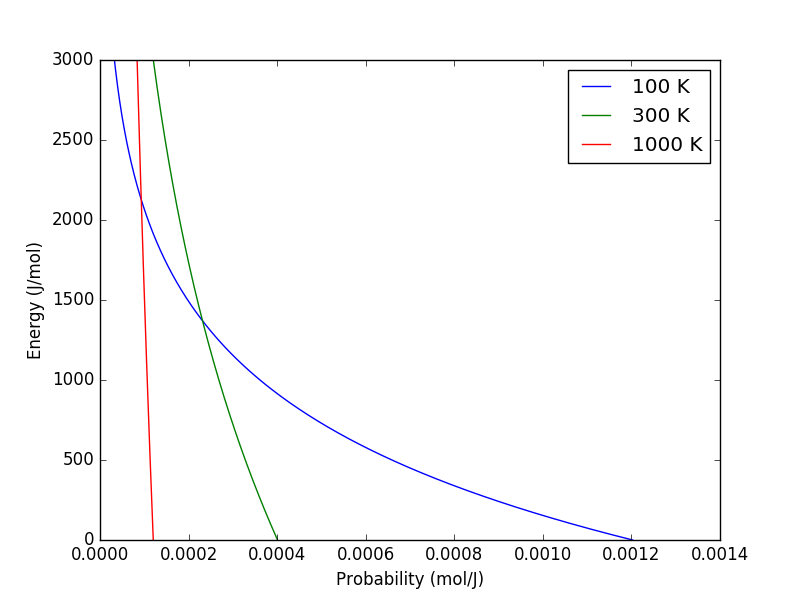
\includegraphics[width=0.5\textwidth]{./Images/Boltzmann.png}
\caption{Boltzmann distribution at various temperatures}
\end{figure}


\begin{figure}[htbp]
\centering
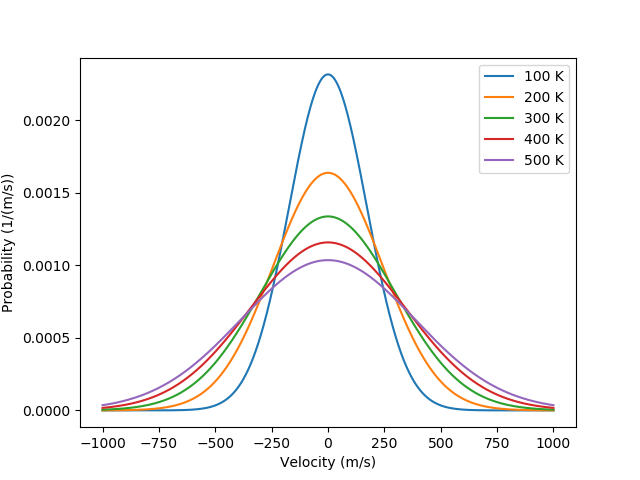
\includegraphics[width=0.5\textwidth]{./Images/MB1D.png}
\caption{One-dimensional (Gaussian) velocities of N\(_2\) gas}
\end{figure}

\begin{figure}[htbp]
\centering
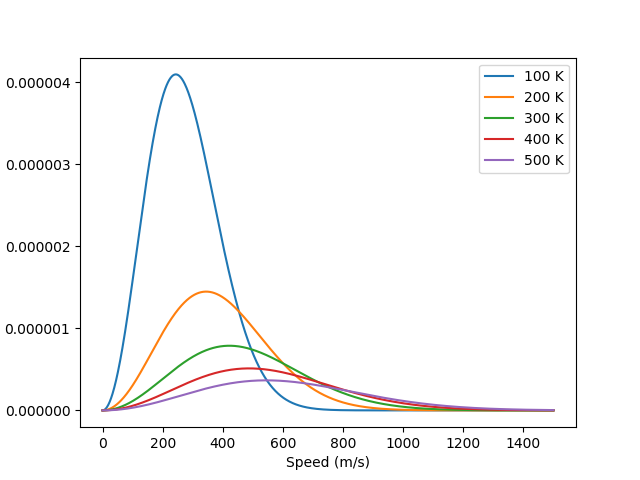
\includegraphics[width=0.5\textwidth]{./Images/MB.png}
\caption{Maxwell-Boltzmann speed distribution of N\(_2\) gas}
\end{figure}

\subsection{Lecture 2: Kinetic theory of gases}
\label{sec:org468349b}
\begin{enumerate}
\item Postulates
\begin{enumerate}
\item Gas is composed of molecules in constant random, thermal motion
\item Molecules only interact by perfectly elastic collisions
\item Volume of molecules is \(<<\) total volume
\end{enumerate}
\item Maxwell-Boltzmann distribution of molecular speeds
\begin{enumerate}
\item Speed \(v=\sqrt{v_x^2+v_y^2+v_z^2}\)
\item \(P_{MB}(v) dv = P_{1D}(v_x) P_{1D}(v_y) P_{1D}(v_z) * \text{degeneracy}(v) dv\)
\item mean speeds \(\propto \sqrt{T}\)
\item mean energy \(U=\frac{3}{2} RT\) and heat capacity \(C_v=\frac{3}{2} R\)
\end{enumerate}
\item Flux and pressure
\begin{enumerate}
\item Velocity flux \(j(v_x) dv_x= v_x \frac{N}{V}P(v_x)dv_x\), molecules /area /time /\(v_x\)
\item Wall collisions, \(J_w\), total collisions /area /time
\item Momentum exchange, pressure, ideal gas law
\end{enumerate}
\item Collisions and mean free path
\begin{enumerate}
\item Collision cross section \(\sigma=\pi d^2\), size of molecule
\item Molecular collisions, \(z\) per molecule and \(z_{\mathrm{AA}}\) per volume
\item Mean free path, \(\lambda\), mean distance between collisions
\end{enumerate}
\end{enumerate}

\begin{figure}[htbp]
\centering
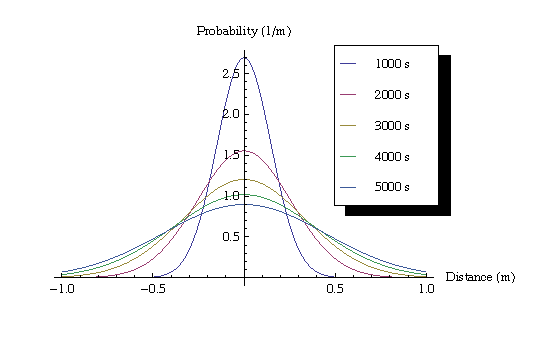
\includegraphics[width=0.6\textwidth]{./Images/Diffusion.pdf}
\caption{Diffusional spreading, \(\sqrt{\langle x^2 \rangle} = \sqrt{2 D t}\)}
\end{figure}

\begin{table} 
\begin{center}
    \caption{Kinetic theory of gases key equations}
    \begin{tabular}{|lr|}
     \hline
 & \\
Boltzmann distribution & $\displaystyle P(E) = g(E) e^{-E/k_BT}$ \\ \ \ \ \ ($g(E)$: degeneracy of
$E$) & \\ 
Maxwell-Boltzmann distribution & $ \displaystyle
P_{\rm MB}(v) = 4\pi v^2 \left( \frac{m}{2\pi k_B T}\right)^{3/2}\exp\left(-\frac{m
    v^2}{2k_B T}\right) $ \\  & \\
Mean and RMS speeds & 

$\displaystyle \langle v \rangle = \left( \frac{8 k_B T}{\pi m} \right)^{1/2} \ \ \ \ \langle v^2
\rangle^{1/2} = \left( \frac{3 k_B T}{m} \right)^{1/2} $ \\  & \\

Pressure & $
\displaystyle \langle P \rangle = \frac{\Delta p}{\Delta t} = m \frac{N}{V}\frac{1}{3}\langle v^2
\rangle = \frac{N k_B T}{V}=\frac{n R T}{V} $ \\ & \\ 

Wall collision frequency &
$ \displaystyle  J_W = \frac{1}{4}\frac{N}{V}\langle v \rangle=\frac{P}{\left( 2 \pi m k_B
    T\right)^{1/2}} $ \\ & \\

Molecular collision frequency &
$ \displaystyle  z=\sqrt{2} \sigma \langle v \rangle\frac{N}{V} = \frac{4\sigma P}{\left( \pi m k_B T
  \right)^{1/2}} $ \\ & \\

Total collisions &
$ \displaystyle z_{AA} = \frac{1}{2} \frac{N}{V} z$ \\ & \\

Mean free path &
$\displaystyle \lambda = \frac{ \langle v \rangle}{z} = \frac{V}{\sqrt{2} \sigma N} $
\\ & \\

Graham's effusion law & $\displaystyle \frac{dN}{dt}=\text{Area}\cdot  J_w \propto 1/m^{1/2} $
\\ & \\
Effusion from a vessel & $\displaystyle P=P_0 e^{-t/\tau}, \tau = \frac{V}{A}\left
  (\frac{2\pi m}{k_B T}\right )^{1/2} $ \\ & \\ 

Self-diffusion constant &
$\displaystyle D_{11} = \frac{1}{3}\langle v \rangle \lambda $ \\ & \\

Diffusion rate &
$\displaystyle \langle x^2 \rangle^{1/2} = \sqrt{2 D t} $\ \ \ \  $\langle r^2 \rangle^{1/2} = \sqrt{6
D t}$ \\ & \\

Einstein-Smoluchowski equation & $\displaystyle D_{11}= \frac{\delta^2}{2\tau}$ \\ & \\

Stokes-Einstein equation for liquids & $\displaystyle D_{11}=\frac{k_BT}{4\pi\eta r}$\ \ \
``Slip'' boundary \\
 & \\
 & $\displaystyle D_\mathrm{Brownian}=\frac{k_BT}{6\pi\eta r}$\ \ \ ``Stick'' boundary \\
\hline
    \end{tabular}
\end{center}
 \end{table}

\subsection{Lecture 3: Transport}
\label{sec:orgd1f3172}
\begin{enumerate}
\item Effusion and Graham's law, \(\text{effusion rate}\propto MW^{-1/2}\)
\item Fick's first law: net flux proportional to concentration gradient
\begin{enumerate}
\item \(j_x = -D \frac{d c}{d x}\)
\item Self-diffusion constant, \(D=\frac{1}{3}\lambda \langle v \rangle\)
\end{enumerate}
\item Knudsen diffusion, \(D=\frac{1}{3}l \langle v \rangle\)
\item Fick's second law: time evolution of concentration gradient
\begin{enumerate}
\item Continuity with no advection: \(\frac{\partial c}{\partial t}
          = -\nabla\cdot \vec{j} + \text{gen}\)
\item One-dimension: \(\frac{d c}{d t} = D \frac{d^2 c}{dx^2}\)
\item Diffusion has Gaussian probability distribution: \(c(x,t)/c_0 = [2 \sqrt{\pi D
          t}]^{-1} \exp(-x^2/4Dt)\)
\end{enumerate}

\item Seeing is believing---Brownian motion
\begin{enumerate}
\item Seemingly random motion of large particles (``dust'') due to ``kicks'' from invisible molecules
\item Einstein receives Nobel Prize for showing:
\begin{enumerate}
\item Motion follows same Gaussian diffusion behavior
\item From steady-state arguments in a field, diffusion constant is ratio of Boltzmann energy, \(k_B T\), to mobility
\item Mobility inversely related to viscosity
\end{enumerate}
\item Stokes-Einstein equation
\item Allows measurement of Avogadro's number, final proof of kinetic theory
\item Similar model for diffusion of liquid molecules, slip boundary
\end{enumerate}

\item Random walk model of diffusion
\begin{enumerate}
\item Binomial distribution
\item Large \(N\) and Stirling approximation
\item Einstein-Smoluchowski relation
\end{enumerate}
\end{enumerate}

\section{Quantum Mechanics: Blurred Lines Between Particles and Waves}
\label{sec:org044e3a2}
\subsection{Lecture 4: Duality and demise of classical physics}
\label{sec:orge3f1bf1}
\subsubsection{Properties of waves}
\label{sec:orgd79f94b}
\begin{enumerate}
\item Traveling waves, standing waves
\item interference, diffraction
\item Expected energy of a classical oscillator, \(\langle \epsilon \rangle _\nu = k_B T\) for all \(\nu\)
\end{enumerate}

\begin{table}
\begin{center}
    \caption{Classical waves}
    \begin{tabular}{|lc|}
     \hline
The wave equation & $\displaystyle \frac{ \partial^2 \Psi(x,t)}{\partial x^2} = \frac{1}{v^2}\frac{\partial^2 \Psi(x,t)}{\partial t^2}$ \\
\\
General solution & \(\Psi(x,t) = A \sin(kx -\omega t)\) \\
Wavelength (distance) & \( \lambda = 2\pi/k \) \\
Frequency (/time) & \( \nu =\omega/2\pi \) \\
Speed & \( v= \lambda \nu \) \\
Amplitude (distance) & \(A\) \\
Energy & \( E \propto A^2 \) \\
Standing wave & \(\Psi(x,t) = A \sin(kx)\cos(\omega t), \quad k =n\pi/a\) \\
\hline
\end{tabular}
\end{center}
\end{table}


\subsubsection{Blackbody radiation}
\label{sec:org814bede}
\begin{enumerate}
\item Hohlraum spectrum (like the sun) empirically observed to obey:
\begin{enumerate}
\item Stefan-Boltzmann law, total irradiance
\item Wien's displacement law
\end{enumerate}
\item Rayleigh-Jeans predicts spectrum using classical physics
\begin{enumerate}
\item standing waves + classical oscillators \(\rightarrow\) ultraviolet catastrophe
\end{enumerate}
\item Planck model
\begin{enumerate}
\item Energy spectrum of oscillators are \emph{quantized}, \(\epsilon_\nu=nh\nu\)
\item Expected energy of a quantized oscillator, \(\langle \epsilon \rangle_\nu = h\nu/\left (
          e^{h\nu/k_BT}-1 \right )\)
\item Correctly reproduces Stefan-Boltzmann and Wien Laws!
\end{enumerate}
\end{enumerate}
\subsubsection{Heat capacities of solids}
\label{sec:orgc52707f}
\begin{enumerate}
\item Law of DuLong and Pettite, \(C_v = 3R\), fails at low \(T\)
\item Einstein model
\begin{enumerate}
\item Atomic vibrations are \emph{quantized}, \(\epsilon_n=nh\nu\)
\item Heat capacity goes to zero at low \(T\)
\end{enumerate}
\end{enumerate}
\subsubsection{Photoelectric effect}
\label{sec:orgaedd5c4}
\begin{enumerate}
\item Stopping potential and work function, \(E_\text{kinetic}=h\nu -W\)
\item Kinetic energy varies with light frequency, number of electrons varies with light intensity
\end{enumerate}
\subsubsection{Compton effect}
\label{sec:orge2b5b07}
\begin{enumerate}
\item light scattering of electrons changes \(\lambda\)
\item Photon properties, \(\epsilon = h\nu, p=h/\lambda\)
\end{enumerate}
\subsubsection{Wave-particle duality}
\label{sec:org5eb6024}
\subsubsection{Rutherford, planetary model of atom}
\label{sec:orgfc545b2}
\begin{enumerate}
\item Inconsistent with Maxwell's equations
\end{enumerate}
\subsubsection{Bohr model of H atom}
\label{sec:orgb1392ab}
\begin{enumerate}
\item Discrete H energy spectrum and Rydberg formala
\item Bohr model (the old quantum mechanics)
\begin{enumerate}
\item Stable electron ``orbits,'' quantized angular momentum
\item Light emission corresponds to orbital jumps, \(\nu=\Delta E/h\)
\item Bohr equations
\item Comparison with Rydberg formula
\item Failure for larger atoms
\end{enumerate}
\end{enumerate}
\subsubsection{de Broglie relation}
\label{sec:orgc002cc8}
\begin{enumerate}
\item \(\lambda=h/p\) \emph{universally}
\item Relation to Bohr orbits
\item Davison and Germer experiment, \(e^-\) diffraction off Ni
\end{enumerate}

\begin{figure}[htbp]
\centering
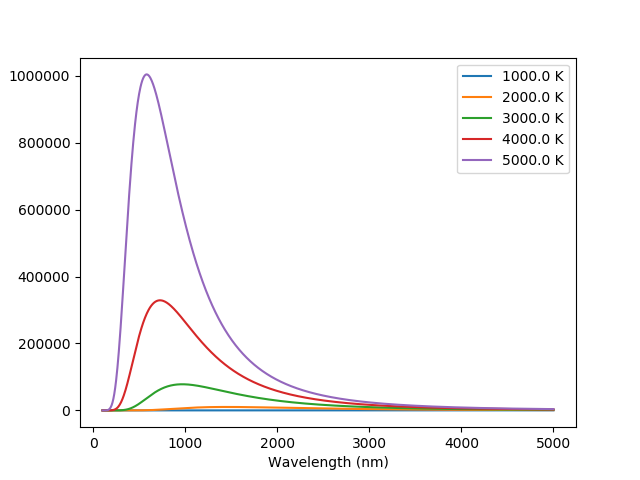
\includegraphics[width=0.5\textwidth]{./Images/BlackBody.png}
\caption{Blackbody irradiance}
\end{figure}
\begin{figure}[htbp]
\centering
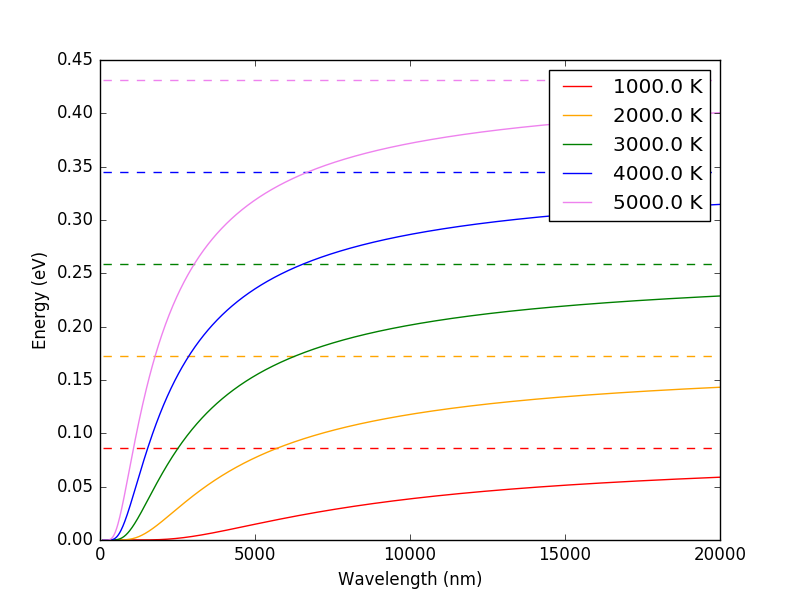
\includegraphics[width=0.5\textwidth]{./Images/Planck.png}
\caption{Average energy of a Planck quantized oscillator}
\end{figure}

\begin{table} 
\begin{center}
    \caption{The new physics}
    \begin{tabular}{|lr|}
     \hline
 & \\
Stefan-Boltzmann Law & $\displaystyle  \int I(\lambda,T)d\lambda = \sigma_\mathrm{SB} T^4$
\\ & \\
Wien's Law & $\displaystyle \lambda_\mathrm{max}T=2897768$ nm K \\
 & \\
Rayleigh-Jeans eq& $\displaystyle I(\lambda,T) = \frac{8\pi}{\lambda^4} k_B T c $ \\ 
& \\
Blackbody irradiance & $\displaystyle I(\lambda, T) =
\frac{8\pi}{\lambda^5}\frac{hc^2}{e^{hc/\lambda k_B T}-1}$ \\ 
& \\
Einstein crystal & $\displaystyle C_v=3R \left(\frac{h\nu}{k_BT}\right )^2\frac{e^{h\nu/k_BT}}{\left
            ( e^{h\nu/k_BT}-1 \right )^2}$ \\
& \\
Photon energy & $\displaystyle \epsilon=h\nu = hc/\lambda $ \\
& \\
Rydberg equation & $\displaystyle \nu = R_H c\left (1/n^2
        -1/k^2 \right)$ \\
& \\
Bohr equations & $\displaystyle l_n=n \hbar$ \\
$\displaystyle n=1,2, \ldots $ & $\displaystyle r_n = n^2 \left ( \frac{4 \pi
    \epsilon_0 \hbar^2}{e^2 m_e} \right ) = n^2 a_0$ \\
 & $\displaystyle E_n =-\frac{m_e e^4}{8\epsilon_0^2
   h^2}\frac{1}{n^2}=-\frac{E_H}{2}\frac{1}{n^2}$ \\ 
 & $\displaystyle p_n =\frac{e^2}{4\pi\epsilon_0}\frac{m_e}{\hbar}\frac{1}{n} =
p_0 \frac{1}{n} $ \\
& \\
de Broglie equation & \[\lambda=\dfrac{h}{p}\] \\
\hline
\end{tabular}
\end{center}
\end{table}

\subsection{Lecture 5: Postulates of quantum mechanics}
\label{sec:orgc6ea5c8}
\subsubsection{Schr\"{o}dinger equation describes wave-like properties of matter}
\label{sec:orgc54dc43}
\subsubsection{Born interpretation}
\label{sec:org52cd0c4}
\begin{enumerate}
\item wavefunction is a probability amplitude
\item wavefunction squared is probability density
\end{enumerate}
\subsubsection{Postulates}
\label{sec:orge5cffa7}
\begin{enumerate}
\item Wavefunction contains all information about a system
\item Operators used to extract that information
\begin{enumerate}
\item QM operators are \emph{Hermitian}
\item Have eigenvectors and real eigenvalues, \(\hat{O}\psi_i=o\psi_i\)
\item Are orthogonal, \(\langle \psi_i | \psi_j \rangle = \delta_{ij}\)
\item Always observe an eigenvalue when making an observation
\end{enumerate}
\item Expectation values
\item Energy-invariant wavefunctions given by Schr\"{o}odinger equation
\item Uncertainty principle
\end{enumerate}
\subsubsection{Particle in a box illustrations}
\label{sec:orgb0b7f9e}

\begin{table} 
\begin{center}
    \caption{\large{Postulates of Non-relativistic Quantum Mechanics}}
   \begin{description}
    \item[Postulate 1:] {{\bf The physical state of a system is completely described by
        its wavefunction $\Psi$.}  In general, $\Psi$ is a complex function of the spatial
      coordinates and time.  $\Psi$ is required to be:}
    \begin{outline}
      \item{Single-valued}
      \item {continuous and twice differentiable}
      \item {square-integrable ($\int \Psi^*\Psi d\tau$ is defined over all finite domains)}
      \item {For bound systems, $\Psi$ can always be normalized such that $\int \Psi^*\Psi d\tau=1$}
    \end{outline}

  \item[Postulate 2:]  To every physical observable quantity $M$ there corresponds a
    Hermitian operator $\hat{M}$.  {\bf The only observable values of $M$ are the
      eignevalues of $\hat{M}$.}
    \begin{center}
    \begin{tabular}[h]{ccc}
      \hline
{\bf Physical quantity} & {\bf Operator} & {\bf Expression} \\
\hline
Position $x,y,z$ & $\hat{x},\hat{y},\hat{z}$ & $x\cdot, y\cdot, z\cdot$ \\ \\
Linear momentum $p_x, \ldots$ & $\hat{p}_x,\ldots $ & $\displaystyle -i\hbar\frac{\partial}{\partial
  x},\ldots $\\
Angular momentum $l_x, \ldots$ & $\hat{p}_x,\ldots $ & $\displaystyle -i\hbar \left
  (y\frac{\partial}{\partial z}-z\frac{\partial}{\partial y}\right ), \ldots $ \\
Kinetic energy $T$ & $\hat{T}$ & $\displaystyle -\frac{\hbar^2}{2m}\nabla^2$ \\
Potential energy $V$ & $\hat{V}$ & $V({\bf r},t)$ \\
Total energy $E$ & $\hat{H}$ & $\displaystyle -\frac{\hbar^2}{2m}\nabla^2+V({\bf r},t)$\\ \\
\hline
    \end{tabular}
  \end{center}
    \item[Postulate 3:] {If a particular observable $M$ is measured many times on many
      identical systems is a state $\Psi$, the average resuts with be the expectation
      value of the operator $\hat{M}$:
      \begin{equation*}
        \langle M \rangle = \int \Psi^* (\hat{M}\Psi)d{\bf\tau}
      \end{equation*}}
    \item[Postulate 4:] {The energy-invariant states of a system are solutions of the equation
        \begin{eqnarray*}
          \hat{H}\Psi({\bf r},t) & = & i\hbar\frac{\partial}{\partial t}\Psi({\bf r},t) \\
          \hat{H} & = & \hat{T}+\hat{V}
        \end{eqnarray*}
      The time-independent, stationary states of the system are solutions to the equation
      \begin{equation*}
        \hat{H}\Psi({\bf r}) = E\Psi(\bf{r})
      \end{equation*}
}
    \item[Postulate 5:] (The {\bf uncertainty principle}.)  Operators that do not commute
      $(\hat{A}(\hat{B}\Psi)\neq\hat{B}(\hat{A}\Psi))$ are called {\em conjugate}.
      Conjugate observables cannot be determined simultaneously to arbitrary accuracy.
      For example, the standard deviation in the measured positions and momenta of
      particles all described by the same $\Psi$ must satisfy $\Delta x\Delta p_x \geq \hbar/2$.
    \end{description}
\end{center}
\end{table}
\subsection{Lecture 6: Particle in a box model}
\label{sec:org21614b6}
\subsubsection{Particle between infinite walls, electron confined in a wire}
\label{sec:org8ce9a71}
\subsubsection{Classical solution, either stationary or uniform bouncing back and forth}
\label{sec:org6668402}
\subsubsection{One-dimesional QM solutions}
\label{sec:org8d445dc}
\begin{enumerate}
\item Schr\"{o}dinder equation and boundary conditions
\item discrete, quantized solutions
\item standing waves, \(\lambda=2 L/n\), \(n-1\) nodes, non-uniform probability
\item \href{http://dx.doi.org/10.1021/jp053496l}{Ho paper}, STM of Pd wire
\item zero point energy and uncertainty
\item correspondence principle
\item superpositions
\end{enumerate}
\subsubsection{Finite walls and tunneling}
\label{sec:org640a292}
\begin{enumerate}
\item Potential well of finite depth \(V_0\)
\item Finite number of bound states
\item Classical region, \(\psi(x) ~ e^{ikx}+e^{-ikx}, k=\sqrt{2mE}/\hbar\)
\item ``Forbidden'' region, \(\psi(x) ~ e^{\kappa x}+e^{-\kappa x},
      \kappa=\sqrt{2m(V_0-E)}/\hbar\)
\item Non-zero probability to ``tunnel'' into forbidden region
\item Tunneling between two adjacent wells: chemical bonding, STM, nanoelectronics
\item H atom tunneling: NH\(_3\) inversion, H transfer, kinetic isotope effect
\end{enumerate}
\subsubsection{Multiple dimensions}
\label{sec:org05575c6}
\begin{enumerate}
\item separation of variables, one quantum number for each dimension
\end{enumerate}
\subsubsection{Introduce Pauli principle for fermions?}
\label{sec:orgbfd5bfb}

\begin{table}[tb]
   \begin{center}
   \caption{Particle-in-a-box model}
    \label{Particle-in-a-box}
\begin{tabular}[h]{|c|}
\hline
 \\
$\displaystyle       V(x) = \left \{
        \begin{array}{rl}
          0 & 0 < x < L \\
          \infty & x \leq 0 \text{ or } x \geq L
        \end{array} \right . $ \\
 \\
$\displaystyle     \psi_n(x) =\sqrt{\frac{2}{L}} \sin \left ( \frac{n\pi x}{L} \right )$
\\ 
 \\
$\displaystyle     E_n =\frac{n^2\pi^2\hbar^2}{2mL^2}, n = 1, 2, ...$ \\
 \\
     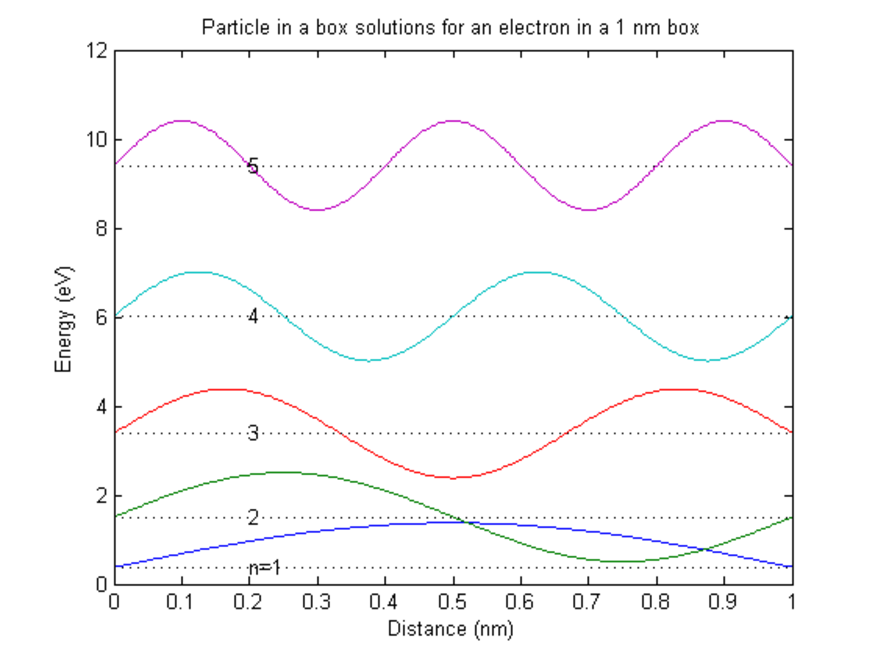
\includegraphics[scale=.6]{Images/PIB} \\       
\hline
\end{tabular}
 \end{center}
\end{table}

\subsection{Lecture 7: Harmonic oscillator}
\label{sec:org1f46efe}
\subsubsection{Classical harmonic oscillator}
\label{sec:orge10a209}
\begin{enumerate}
\item Hooke's law, \(F=-k(x-x_0)\), \(k\) spring constant
\item Continuous sinusoidal motion
\item \(x(t)=A \sin(\frac{k}{\mu})^{1/2}t, \nu=\frac{1}{2\pi}(\frac{k}{\mu})^{1/2}, E=\frac{1}{2}kA^2\)
\item Exchanging kinetic and potential energies
\end{enumerate}
\subsubsection{Quantum harmonic oscillator}
\label{sec:org5ec7f3a}
\begin{enumerate}
\item Schr\"{o}dinger equation and boundary conditions
\item Solutions like P-I-A-B + tunneling at boundaries
\item Zero-point energy and uniform energy ladder
\item Parity operator and even/odd symmetry:  \(\langle x \rangle =0\)
\item Recursion relations: \(\langle x^2 \rangle =
      \alpha^2 (v+1/2), \langle V(x) \rangle = \frac{1}{2} h\nu (v+\frac{1}{2})\)
\item Virial theorem
\item Classical turning point and tunneling
\item Classical limiting behavior
\end{enumerate}
\subsubsection{HCl example}
\label{sec:orgb208577}
\begin{enumerate}
\item Reduced mass, \(\frac{1}{\mu}=\frac{1}{m_A}+\frac{1}{m_B}\)
\item ZPE, energy spacing in IR, Boltzmann probabilities
\end{enumerate}

\begin{table}[]
   \begin{center}
   \caption{Harmonic oscillator model}
    \label{Harmonic-oscillator}
\begin{tabular}[h]{|c|}
\hline
 \\
$\displaystyle       V(x) = \frac{1}{2} k x^2, -\infty < x < \infty $ \\
 \\
$\displaystyle     \psi_v(x) = N_v H_v(x/\alpha)e^{-x^2/2\alpha^2}, v = 0, 1, 2, \ldots $ \\
\\
$\displaystyle \alpha=(\hbar^2/\mu k)^{1/4}, N_v=(2^vv!\alpha\sqrt{\pi})^{-1/2} $ \\
 \\
\underline{Hermite polynomials} \\
$\displaystyle H_0(y) =1$\\
$\displaystyle H_1(y) = 2y$\\
$\displaystyle H_2(y) = 4y^2-2$\\
$\displaystyle H_{n+1}(y) = 2 y H_n(y) -2 n H_{n-1}(y)$\\
 \\
$\displaystyle     \nu =\frac{1}{2\pi}\sqrt\frac{k}{\mu}$ \\
$\displaystyle     E_v=(v+\frac{1}{2})h \nu, v=0, 1, 2, ...$ \\
 \\
     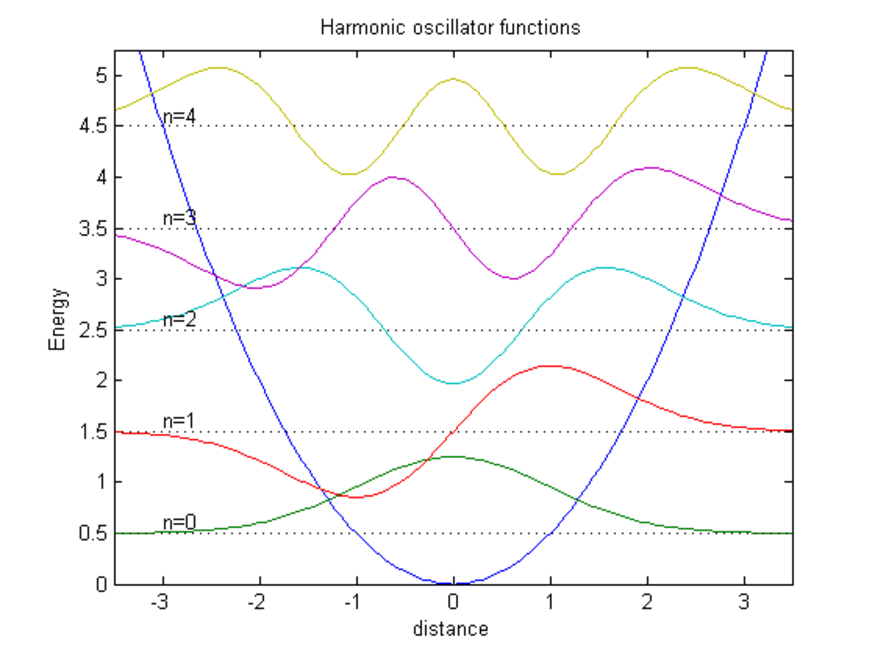
\includegraphics[scale=.6]{Images/HO} \\       
\hline
\end{tabular}
 \end{center}
\end{table}

\subsection{Lecture 8: Rigid Rotor}
\label{sec:orgf79bfab}
\subsubsection{Classical rigid rotor}
\label{sec:org3145bb9}
\begin{enumerate}
\item Compare rotation about an axis vs linear motion
\item Moment of intertia \(I=\mu r^2\)
\item Angular momentum, \(\mathbf{l} = I \mathbf{\omega} = \mathbf{r}\times \mathbf{p}\), \(T= l^2/2I\) 
\begin{enumerate}
\item Angular momentum and energy continuous variables
\end{enumerate}
\end{enumerate}
\subsubsection{Quantum rotor in a plane}
\label{sec:org8706df7}
\begin{enumerate}
\item Angular momentum and kinetic energy operators in polar coordinates,
\(\hat l_z = -i\hbar \frac{d}{d\phi}\)
\item Eigenfunctions degenerate, cw and ccw rotation
\item No zero point energy
\item Angular momentum eignefunctions, \(l_z = m_l \hbar\)
\item Energy superpositions and localization
\end{enumerate}

\begin{table}[tbh]
   \begin{center}
   \caption{2-D rigid rotor model}
    \label{Rigid rotor}
\begin{tabular}[h]{|c|}
\hline
 \\
$\displaystyle       V(\phi) = 0, 0 \leq \phi \leq 2\pi $ \\
 \\
$\displaystyle \hat H = -\frac{\hbar^2}{2 I} \frac{\partial^2}{\partial
  \phi^2},\ \ \ \ \ I=\mu R^2
$\\
\\
$\displaystyle     \psi_{m_l}(\phi) = \frac{1}{\sqrt{2\pi}} e^{-i m_l \phi}, m_l
= 0, \pm 1, \pm 2, \ldots $ \\
\\
$\displaystyle     E_{m_l}=\frac{\hbar^2}{2 I}m_l^2$ \\
 \\
$\displaystyle L_z = m_l \hbar$ \\
\\
     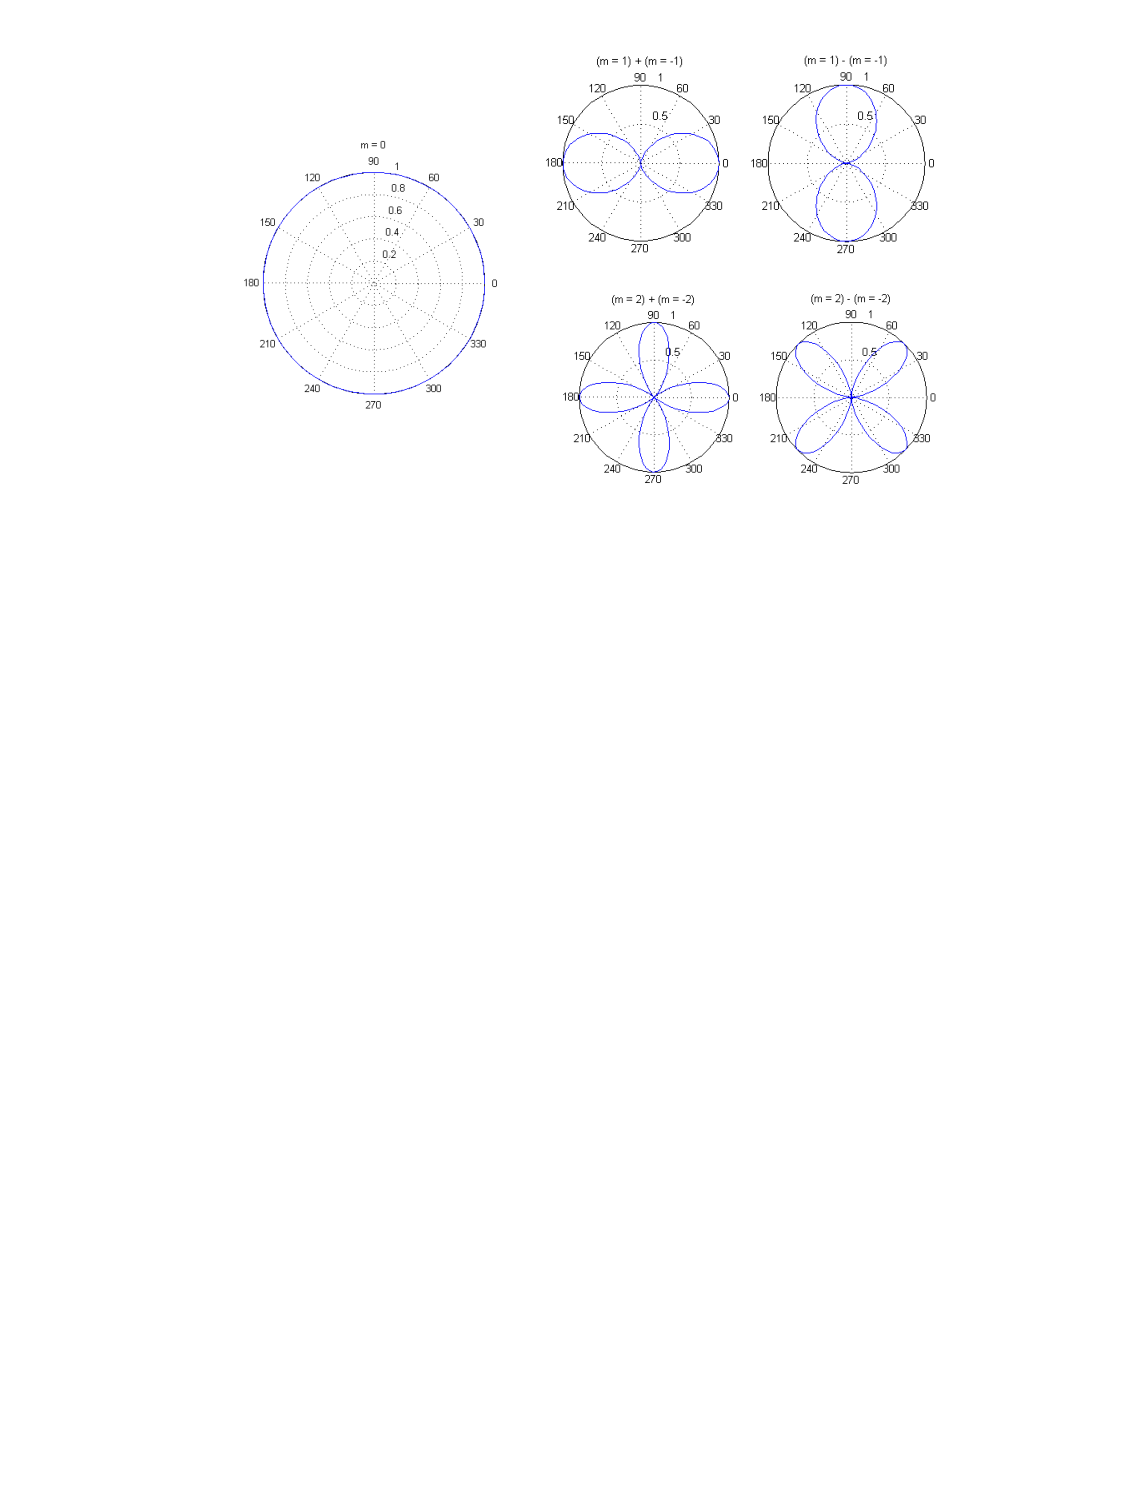
\includegraphics[scale=1]{Images/2Drotor.pdf} \\       
\hline
\end{tabular}
 \end{center}
\end{table}

\subsubsection{Quantum rotor in 3-D}
\label{sec:orgfbdf88f}
\begin{enumerate}
\item Angular momentum and kinetic energy operators in spherical coordinates
\item Spherical harmonic solutions, \(Y_{lm_l}\)
\item Azimuthal QN \(l=0, 1, \ldots\)
\item Magnetic QN \(m_l = -l, -l+1, ..., l\)
\item Energy spectrum, \(2 l + 1\) degeneracy
\item Vector model - can only know total total \(|L|\) and \(L_z\)
\item Wavefunctions look like atomic orbitals, \(l\) nodes
\end{enumerate}

\begin{table}
   \begin{center}
   \caption{3-D rigid rotor model}
    \label{3-D Rigid rotor}
\begin{tabular}[h]{|c|}
\hline
 \\
$\displaystyle       V(\theta,\phi) = 0, 0 \leq \phi \leq 2\pi, 0 \leq \theta <
\pi$ \\
 \\
$\displaystyle     \hat L^2 = -\hbar^2 \left [
  \frac{1}{\sin^2\theta}\frac{\partial^2}{\partial \phi^2}+\frac{1}{\sin
    \theta}\frac{\partial}{\partial \theta}\left ( \sin \theta
    \frac{\partial}{\partial \theta}\right ) \right ] $ \\
\\
$\displaystyle \hat H_\text{rot} = \frac{1}{2 I} \hat L^2$ \\
\\
$\displaystyle     Y_{lm_l}(\theta,\phi)=N_l^{|m|}P_l^{|m|}(\cos(\theta))e^{im_l\phi}$ \\
\\
$\displaystyle l = 0, 1, 2, \ldots, \ \ \ \ \ \ m_l = 0,\pm 1, \ldots, \pm l$
\\
\\
$\displaystyle     E_{l}=\frac{\hbar^2}{2 I}l(l+1)$ \\
 \\
$\displaystyle |L| = \hbar \sqrt{l(l+1)}, L_z = m_l \hbar $ \\
% \\
%     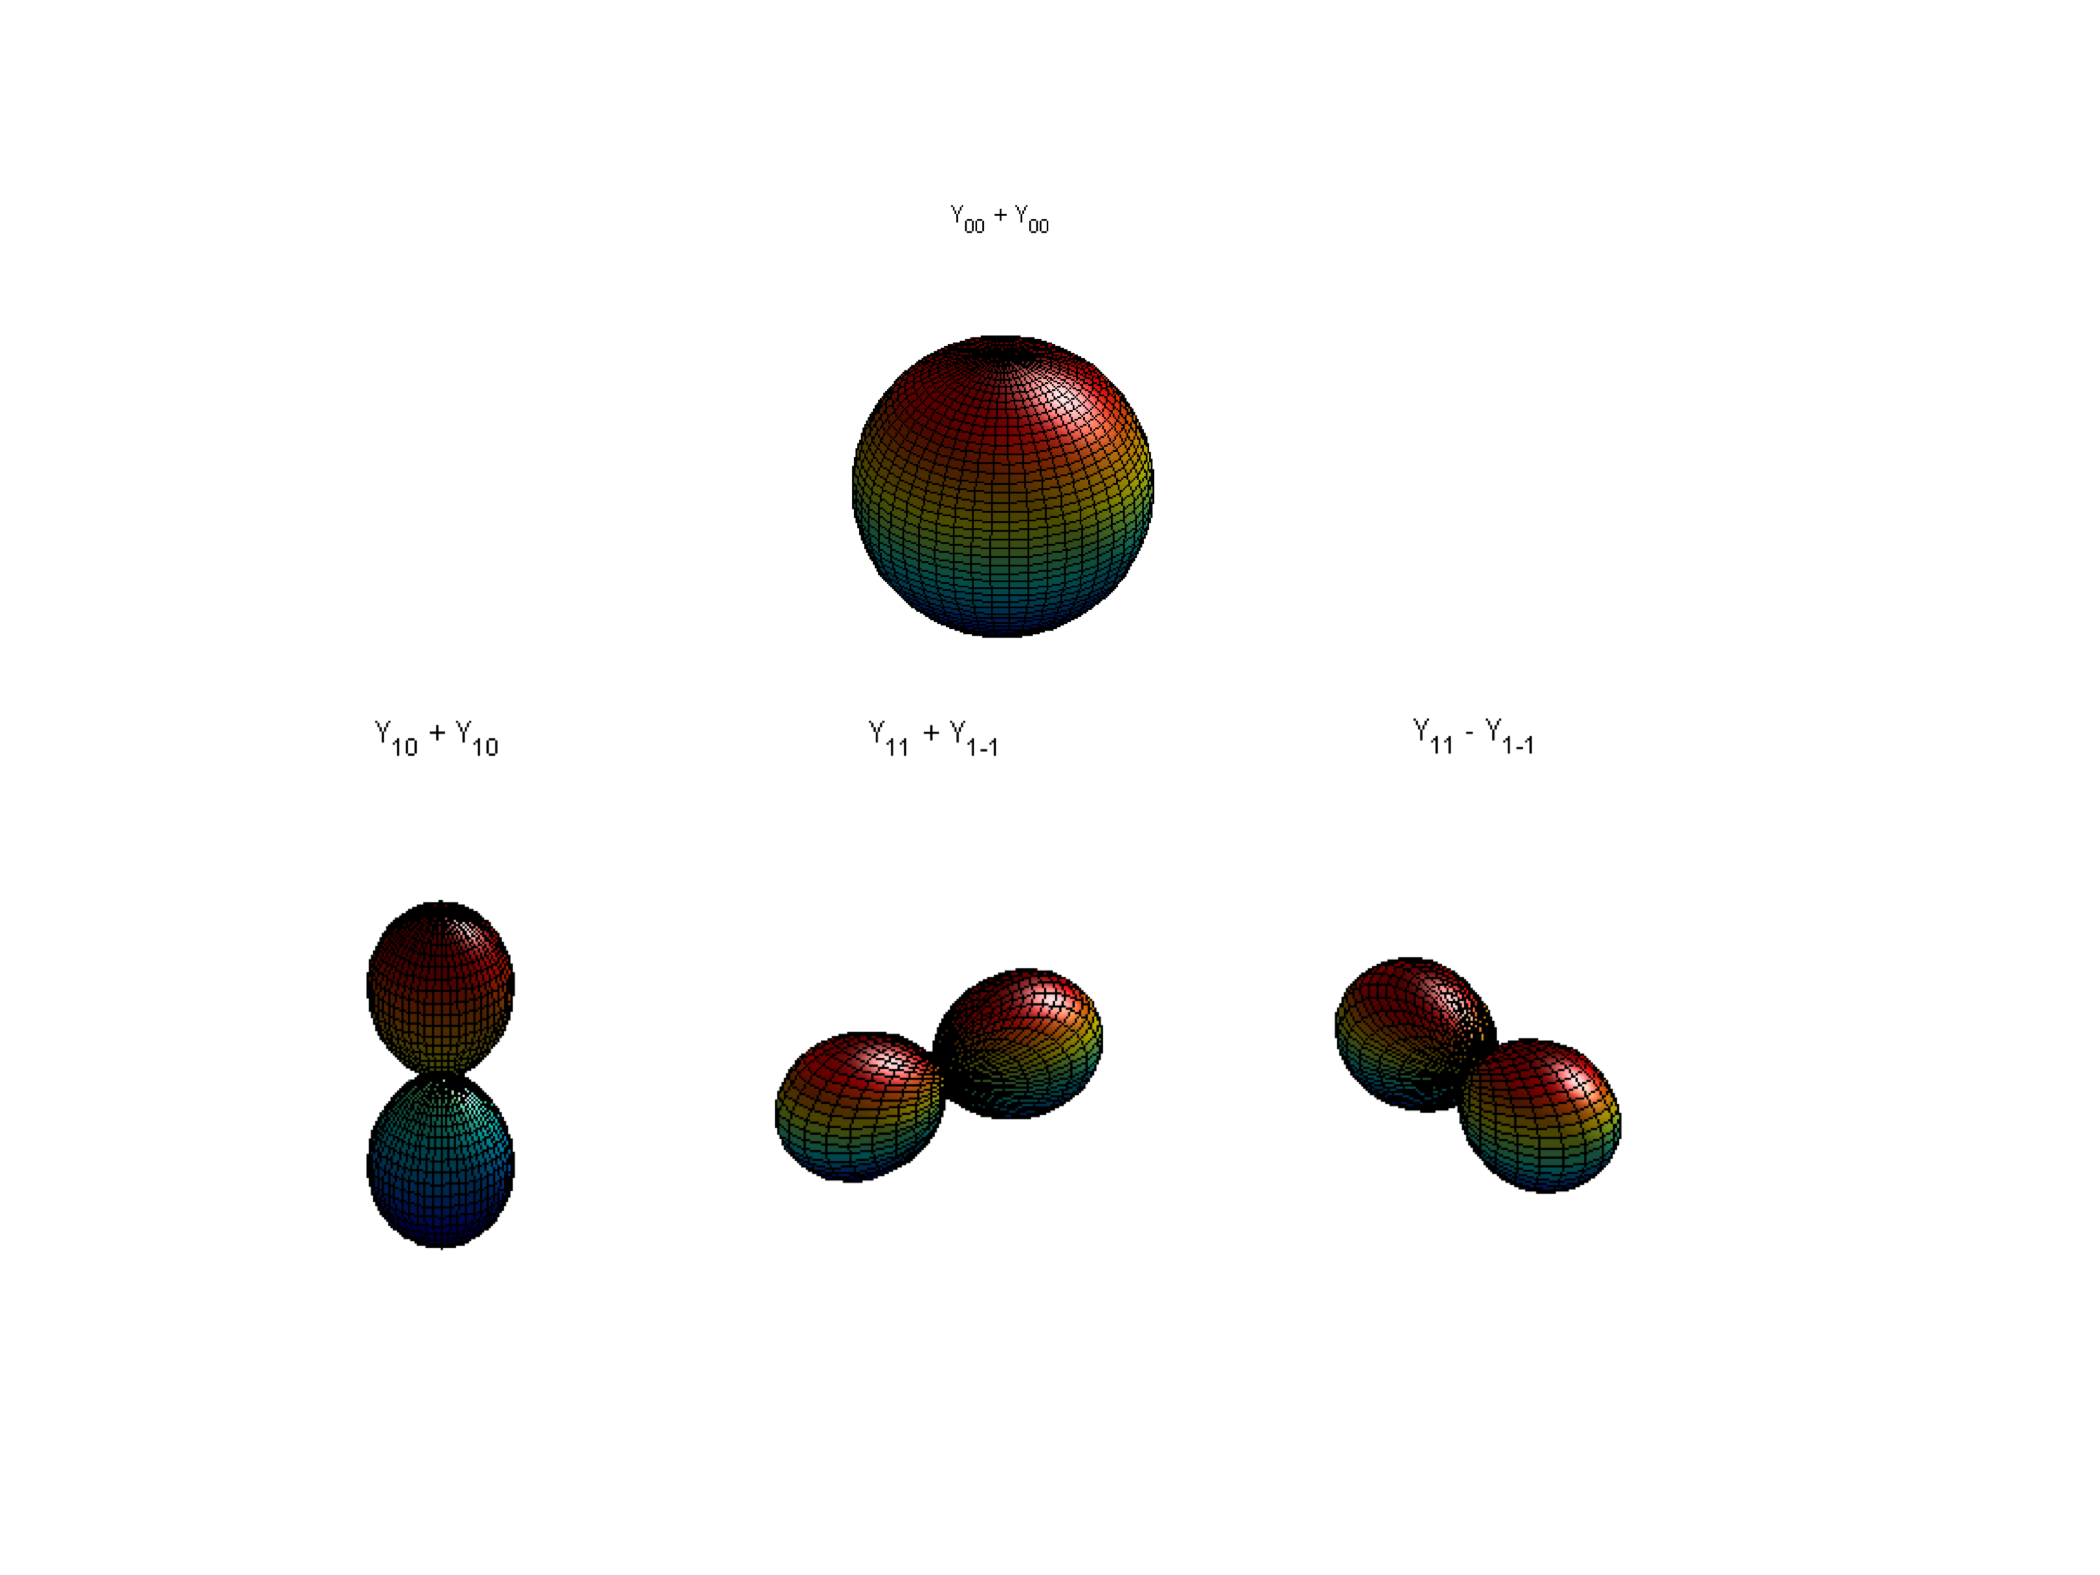
\includegraphics[scale=0.4]{Images/3Drotor.png} \\       
\hline
\end{tabular}
 \end{center}
\end{table}


\begin{figure}

\includegraphics[scale=0.4]{./Images/s.png}
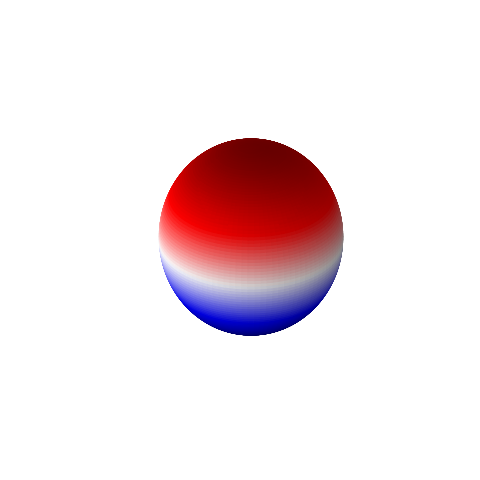
\includegraphics[scale=0.4]{./Images/p.png}
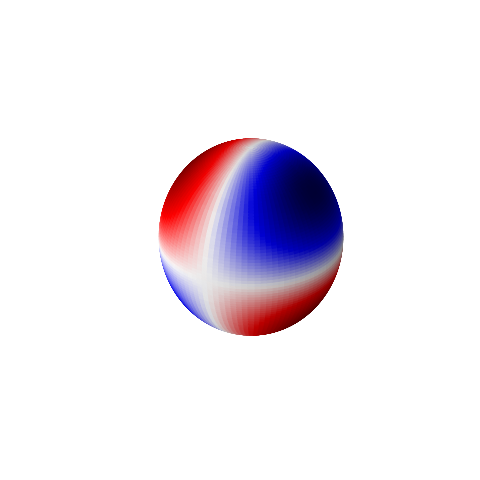
\includegraphics[scale=0.4]{./Images/d.png}
\caption{Pythonic $s$ ($l = 0$), $p$ ($l=1$), and $d$ ($l=2$) spherical harmonics. Color scale from red to white to blue corresponds to positive to zero to negative sign of wavefunction.}
\end{figure}

\subsubsection{Particle angular momentum}
\label{sec:orge8e6a90}
\begin{enumerate}
\item Fermions, mass, half-integer spin
\begin{enumerate}
\item Electron, \(s=1/2, m_s=\pm 1/2\)
\end{enumerate}
\item Bosons, force-carrying, integer spin
\end{enumerate}
\subsection{Lecture 9: Spectroscopy}
\label{sec:org3dce52a}
\subsubsection{Spectroscopy is quantitative measurement of interaction of light with matter}
\label{sec:orgcd8387d}
\begin{enumerate}
\item Observed \(I(\nu)/I(\nu_0)\)
\item Bohr condition, \(|E_f-E_i|/h=\nu =c\tilde{\nu}=c/\lambda\)
\item Intensities determined by state populations and transition probabilities
\end{enumerate}
\subsubsection{Einstein coefficients}
\label{sec:orge33f4fc}
\begin{enumerate}
\item Stimulated absorption, \(dn_1/dt= -n_1 B\rho(\nu)\)
\item Stimulated emission, \(dn_2/dt= -n_2 B\rho(\nu)\)
\item Spontaneous emission, \(dn_2/dt=-n_2 A, A=\left ( \frac{8\pi h
              \nu^3}{c^3}\right )B\)
\item \(1/A=\) lifetime
\end{enumerate}
\subsubsection{Transition probability}
\label{sec:org0aa01b2}
\begin{enumerate}
\item Einstein coefficient \(B_{if}=\frac{|\mu_{if}|^2}{6\epsilon_0\hbar^2}\)
\item Classical electric dipole, \(\overrightarrow{\mu}=q \cdot
          \overrightarrow{l}\), quantum dipole operator \(\hat\mu = e\cdot \overrightarrow{r}\)
\item Transition dipole moment, \(\mu_{if} = \left(
        \frac{d\mu}{dx}\right ) \langle \psi_i|\hat\mu |\psi_f \rangle\)
\item Selection rules---conditions that make \(\mu_{if}\) non-zero,
``allowed'' vs ``forbidden'' transitions
\end{enumerate}
\subsection{Lecture 10: Vibrational and rotational spectroscopy}
\label{sec:org450a54e}
\subsubsection{Diatomic rotational spectroscopy}
\label{sec:org0b9f7d5}
\begin{enumerate}
\item Rotational constant \(B = \hbar/4\pi I c\) cm\(^{-1}\), \(I=\mu R^2\)
\item Gross selection rule: dynamic dipole moment non-zero (heteronuclear, not homonuclear)
\item Specific selection rule: \(\Delta l=\pm 1\), \(\Delta m_l=0, \pm1\)
\item \(\Delta \tilde E_l  = 2B(l+1)\) cm\(^{-1}\)
\item Rotational state populations
\end{enumerate}
\subsubsection{Diatomic vibrational transitions}
\label{sec:org63c8ad7}
\begin{enumerate}
\item Gross selection rule: dynamic dipole \(d\mu/dx\) non-zero
\item Homo- vs. heteronuclear
\item Specific selection rule: dipole integral \(\langle \psi_v|\hat\mu|\psi_{v^\prime} \rangle =0\)
unless \(\Delta v = \pm 1\)
\item Allowed \(\Delta E = h\nu\)
\item Boltzmann distribution implies \(v=1\) states dominate at normal \(T\)
\end{enumerate}
\subsubsection{Raman spectroscopy}
\label{sec:org3e67b47}
\begin{enumerate}
\item Shine in light of arbitrary frequency \(\tilde{\nu_0}\), mostly get out the same
\item Some light comes out at \(\tilde{\nu_0}-\tilde{\nu}\) (Stoke's line)
\item Some light comes out at \(\tilde{\nu_0}+\tilde{\nu}\) (anti-Stoke's line)
\item Gross selection rule: dynamic polarizability non-zero (homonuclear, not heteronuclear)
\end{enumerate}
\subsubsection{Anharmonicity, Morse potential}
\label{sec:org9d52bf1}
\subsubsection{Vibration-rotation spectroscopy}
\label{sec:orge74a9eb}
\begin{enumerate}
\item Harmonic oscillator + rigid rotor
\item Selection rules: \(\Delta v = \pm 1, \Delta l=\pm 1\)
\item \(R\) branch: \(\Delta \tilde E  = \tilde \nu + 2B(l+1), \Delta l = 1\)
\item \(P\) branch: \(\Delta \tilde E = \tilde \nu - 2B(l), \Delta l = -1\)
\end{enumerate}
\begin{figure}[htbp]
\centering
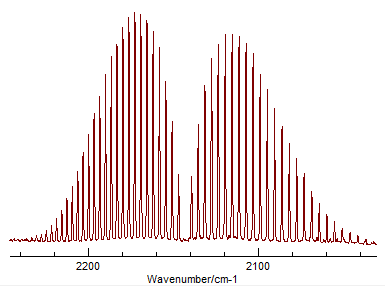
\includegraphics[width=0.5\textwidth]{./Images/CO-rovib.png}
\caption{Rovibrational spectrum of carbon monoxide}
\end{figure}
\subsubsection{Polyatomic vibrational spectroscopy}
\label{sec:org08b11e5}
\begin{enumerate}
\item Polyatomics, \(3n-6\) (\(3n-5\) for linear polyatomic) vibrational modes
\item Selection rules and degeneracies affect number of observed features
\item CO\(_2\) example
\end{enumerate}
\subsubsection{Polyatomic rotational spectroscopy}
\label{sec:orgfb9bd3b}
\begin{enumerate}
\item Three distinct moments of intertia (\(I_x, I_y, I_z\))
\item Spectra more complex
\end{enumerate}
\subsection{Lecture 11: Hydrogen atom}
\label{sec:orgb64c12c}
\subsubsection{Schr\"{o}dinger equation}
\label{sec:org8e629d6}
\begin{enumerate}
\item Spherical coordinates and separation of variables
\item Coulomb potential \(v_\mathrm{Coulomb}(r)=-\frac{e^2}{4\pi\epsilon_0}\frac{1}{r}\)
\item Centripetal potential  \(v=\hbar^2\frac{l(l+1)}{2\mu r^2}\)
\end{enumerate}
\begin{table}[]
   \begin{center}
   \caption{Hydrogen atom}
    \label{Hydrogen atom}
\begin{tabular}[h]{|c|}
\hline
 \\
$\displaystyle       V(r) = -\frac{e^2}{4\pi\epsilon_0}\frac{1}{r}, 0 < r< \infty$ \\
 \\
$\displaystyle     \hat H = -\frac{\hbar^2}{2m_e}\frac{1}{r^2}\left [
  \frac{\partial}{\partial r}r^2\frac{\partial}{\partial r} + \hat L^2 \right ] +V(r)$ \\
\\
$\displaystyle \psi(r,\theta,\phi) = R(r)Y_{l,m_l}(\theta,\phi) $ \\
\\
$\displaystyle   \left \{ -\frac{\hbar^2}{2m_e}\frac{1}{r^2}
            \frac{d}{d r} \left ( r^2 \frac{d}{dr}\right ) + \frac{\hbar^2
              l(l+1)}{2 m_e r^2}
          -\frac{e^2}{4\pi\epsilon_0}\frac{1}{r}\right \} R(r) = E R(r) $ \\
\\
$\displaystyle R_{nl}(r) = N_{nl} e^{-x/2} x^l L_{nl}(x),\ \ \  x = \frac{2 r}{n a_0} $
\\
$\displaystyle P_{nl}(r) = r^2 R_{nl}^2 $
\\
\\
$\displaystyle n = 1, 2, \ldots,\ \  l = 0, \ldots, n-1 \ \ m_l = 0,\pm 1, \ldots, \pm l$
\\
\\
$\displaystyle N_{nl} = \sqrt{\left ( \frac{2}{na_0}\right )^3 \frac{(n-l-1)!}{2n(n+l)!}}$
\\
\\
$\displaystyle L_{10} = L_{21} = L_{32} = \ldots =1 \quad L_{20} = 2 - x \quad L_{31} = 4-x$
\\
\\
\\
$\displaystyle     E_{n}=-\frac{1}{2}\frac{\hbar^2}{m_e a_0^2}\frac{1}{n^2} =-\frac{E_H}{2}\frac{1}{n^2}$ \\
 \\
$\displaystyle |L| = \hbar \sqrt{l(l+1)}, L_z = m_l \hbar $ \\
\\
$\displaystyle \langle r \rangle = \left \{ \frac{3}{2} n^2 - \frac{1}{2} l(l+1) \right \} \frac{a_0}{Z} $ \\
\\
%%     \includegraphics[scale=0.4]{Images/H_atom} \\       
\hline
\end{tabular}
 \end{center}
\end{table}

\subsubsection{Solutions}
\label{sec:orgb02e0f1}
\begin{enumerate}
\item \(\psi(r,\theta,\phi)=R_{nl}(r)Y_{lm}(\theta,\phi)\)
\item Principle quantum number \(n=1,2,\ldots\)
\begin{enumerate}
\item \(K\), \(L\), \(M\), \(N\), \ldots{} shells
\item \(n-1\) radial nodes
\end{enumerate}
\item Azimuthal quantum number \(l=0,1,...,n-1\)
\begin{enumerate}
\item \(s\), \(p\), \(d\), \ldots{} orbital sub-shells
\item \(l\) angular nodes
\end{enumerate}
\item Magnetic quantum number \(m_l=-l,-l+1,...,l\)
\item Spin quantum number \(m_s=\pm 1/2\)
\item Energy spectrum and populations
\item Electronic selection rules
\begin{enumerate}
\item \(\Delta l=\pm 1 \quad \Delta m_s =0 \quad \Delta m_l = 0,\pm 1\)
\end{enumerate}
\item Wavefunctions = ``orbitals''
\item Integrate out angular components to get radial probability function \(P_{nl}(r)=r^2 R_{nl}^2(r)\)
\begin{enumerate}
\item \(\langle r\rangle = \int r P_{nl}(r) dr = \left(\frac{3}{2}n^2-l(l+1)\right)a_0\)
\end{enumerate}
\end{enumerate}



\begin{figure}[htbp]
\centering
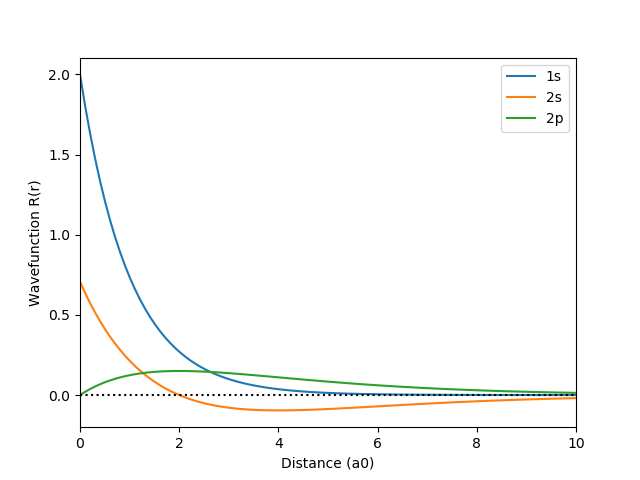
\includegraphics[width=0.75\textwidth]{./Images/H-R.png}
\caption{H atom radial wavefunctions}
\end{figure} 
\begin{figure}[htbp]
\centering
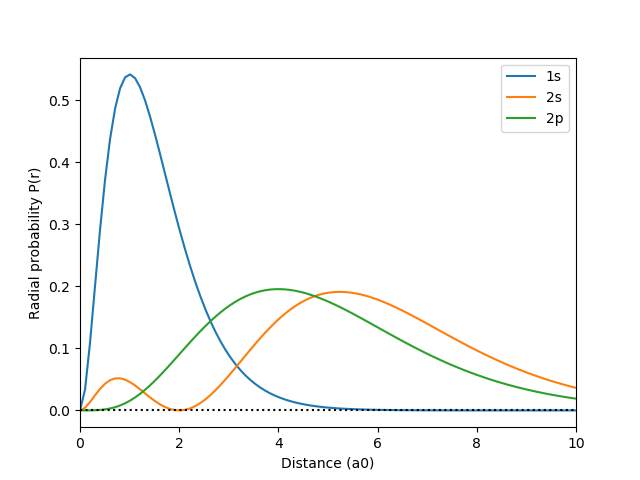
\includegraphics[width=0.75\textwidth]{./Images/H-P.png}
\caption{H atom radial probability}
\end{figure} 

\subsubsection{\emph{Variational principle}}
\label{sec:org71a109b}
\begin{enumerate}
\item Solutions of Schr\"{o}dinger equation always form a complete set
\item True wavefunction energy is therefore lower bound on energy of any trial wavefunction
\end{enumerate}
\[\langle \psi_\text{trial}^\lambda | \hat{H} | \psi_\text{trial}^\lambda\rangle =E_\text{trial}^\lambda \geq E_0\]
\begin{enumerate}
\item Optimize wavefunction with respect to variational parameter
\end{enumerate}
\[ \left ( \frac{\partial \langle \psi_\text{trial}^\lambda | \hat{H} | \psi_\text{trial}^\lambda\rangle}{\partial\lambda} \right ) = 0 \rightarrow \lambda_\text{opt} \] 

\subsection{Lecture 12: Many-electron atoms}
\label{sec:org86f11ff}
\subsubsection{Many-electron problem, Schr\"{o}dinger equation not exactly solvable}
\label{sec:org35e3241}
\begin{enumerate}
\item \(e^- -e^-\) interaction terms prevent separation of variables
\item Independent electron model basis of all solutions, describes each electron by its own wavefunction, or ``orbital''
\end{enumerate}
\subsubsection{Qualitative solutions}
\label{sec:orgd4a2d74}
\begin{enumerate}
\item \(\psi_i\) look like H atom orbitals,  labeled by same quantum numbers
\item \emph{Aufbau principle}: ``Build-up'' electron configuration by adding electrons into H-atom-like orbitals, from bottom up
\item \emph{Pauli exclusion principle}: Every electron in atom must have a unique set of quantum numbers, so only two per orbital (with opposite spin)
\item \emph{Pauli exclusion principle (formally)}: The wavefunction of a multi-particle system must be anti-symmetric to coordinate exchange if the particles are fermions, and symmetric to coordinate exchange if the particles are bosons
\item \emph{Hund's rule}: Electrons in degenerate orbitals prefer to be spin-aligned.  Configuration with highest \emph{spin multiplicity} is the most preferred
\end{enumerate}
\subsubsection{Structure of the periodic table}
\label{sec:org14a7923}
\begin{enumerate}
\item Electrons in different subshells experience different effective nuclear charge \(Z_\mathrm{eff} = Z - \sigma_{nl}\)
\item Inner (``core'') shells not shielded well at
\item Inner shell electrons ``shield'' outer electrons well
\item Within a shell, \(s\) shielded less than \(p\) less than \(d\) \ldots{}, causes degeneracy to break down
\item Electrons in same subshell shield each other poorly, causing ionization energy to increase across the subshell
\end{enumerate}
\subsubsection{Quantitative solutions}
\label{sec:org2c9aca1}
\begin{enumerate}
\item Schr\"{o}dinger equation
\[\hat H \Psi({\bf r}_1, {\bf r}_2,...)=E \Psi({\bf r}_1, {\bf r}_2,...)\]
\[\hat H = \sum_i \hat h_i + \frac{e^2}{4 \pi
          \epsilon_0}\sum_i\sum_{j>i}\frac{1}{|{\bf r}_i-{\bf r}_j|}\]
\[\hat h_i = -\frac{\hbar^2}{2m_e}\nabla^2_i-\frac{Z
          e^2}{4\pi\epsilon_0}\frac{1}{|{\bf r}_i|}\]
\item Construct candidate many-electron wavefunction \(\Psi\) from one
 electron wavefunctions (mathematical details vary with exact approach)
\[\Psi({\bf r}_1, {\bf r}_2,...)\approx \psi_1({\bf
            r}_1)\psi_2({\bf r}_2)...\psi_n({\bf r}_n)\]
\item Calculate expectation value of \(E\) of approximate model and apply
\emph{variational principle} to find equations that describe ``best'' (lowest
 total energy) set of \(\psi_i\)
 \[\frac{\partial E}{\partial \psi_i}=0 \ \ \ \forall i\]
 \[\hat f\psi=\left\{\hat h + \hat v_\mathrm{Coul}[\psi_i] + \hat
            v_\mathrm{ex}[\psi_i]+\hat v_\mathrm{corr}[\psi_i] \right\}\psi=\epsilon\psi\]
 \[E=\sum_i \epsilon_i-\frac{1}{2}\langle \Psi |\hat v_\mathrm{Coul}[\psi_i] + \hat
            v_\mathrm{ex}[\psi_i]+\hat v_\mathrm{corr}[\psi_i]|\Psi \rangle\]
\item Motivate as equation for an electron moving in a ``field'' of
other electrons, adding an electron to a known set of \(\psi_i\)
\end{enumerate}
\subsubsection{Electron-electron interactions}
\label{sec:org64a8c17}
\begin{enumerate}
\item Coulomb (\(\hat v_\mathrm{Coul}\)): classical repulsion between distinguishable electron ``clouds''
\item Exchange (\(\hat v_\mathrm{ex}\)): accounts for electron indistinguishability (Pauli principle for fermions).  Decreases Coulomb repulsion because electrons of like spin intrinsically avoid one another
\item Correlation (\(\hat v_\mathrm{corr}\)): decrease in Coulomb repulsion due to dynamic ability of electrons to avoid one another; ``fixes'' orbital approximation
\item General form of exchange potential is expensive to calculate; general form of correlation potential is unknown
\end{enumerate}
\subsubsection{Popular models}
\label{sec:org5af1c15}
\begin{enumerate}
\item \emph{Hartree model}: Include only classical Coulomb repulsion \(\hat v_\mathrm{Coul}\)
\item \emph{Hartree-Fock model}: Include Coulomb and exchange
\item \emph{Density-functional theory} (DFT): Include Coulomb and
approximate expressions for exchange and correlation
\item All the potential terms \(\hat v\) depend on the solutions, so equations
must be solved \emph{iteratively} to \emph{self-consistency}
\end{enumerate}
\subsubsection{DFT calculations on atoms}
\label{sec:org4513304}
\begin{enumerate}
\item See \url{http://www.chemsoft.ch/qc/fda.htm}
\end{enumerate}

\begin{table}[]
   \caption{Numerical DFT Solutions for Atoms }
\begin{tabular}{cc}
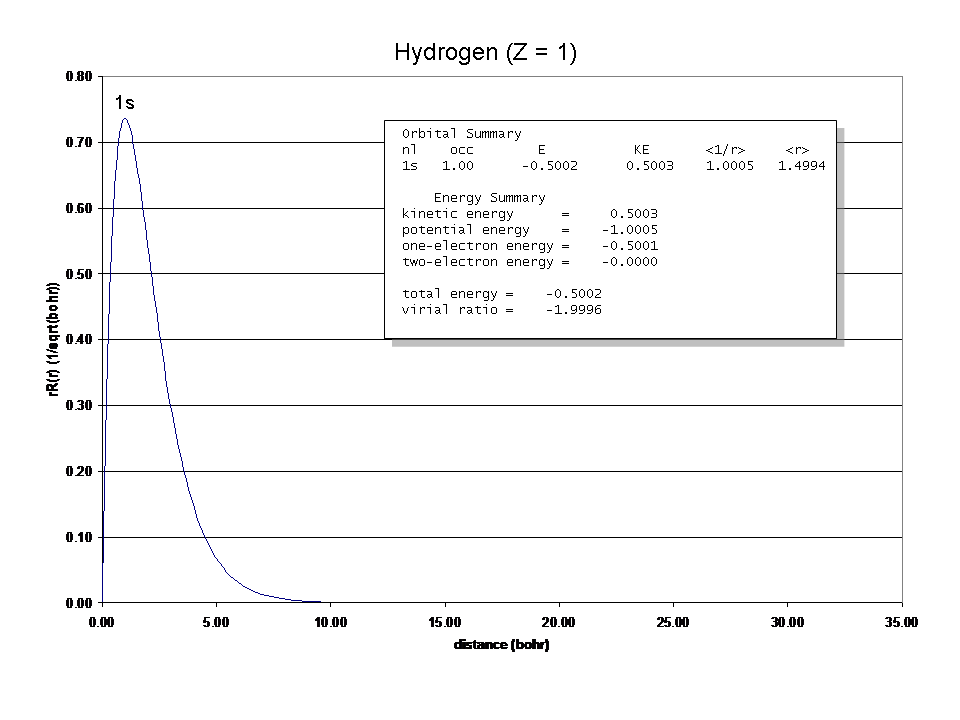
\includegraphics[scale=0.33]{Images/Slide1.png} & 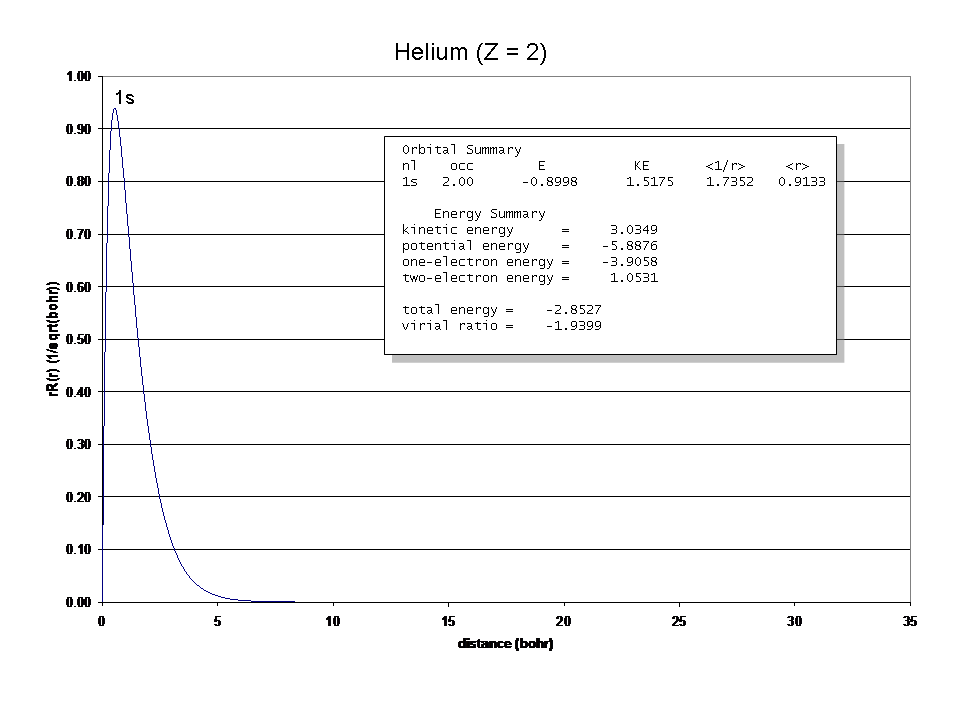
\includegraphics[scale=0.33]{Images/Slide2.png} \\
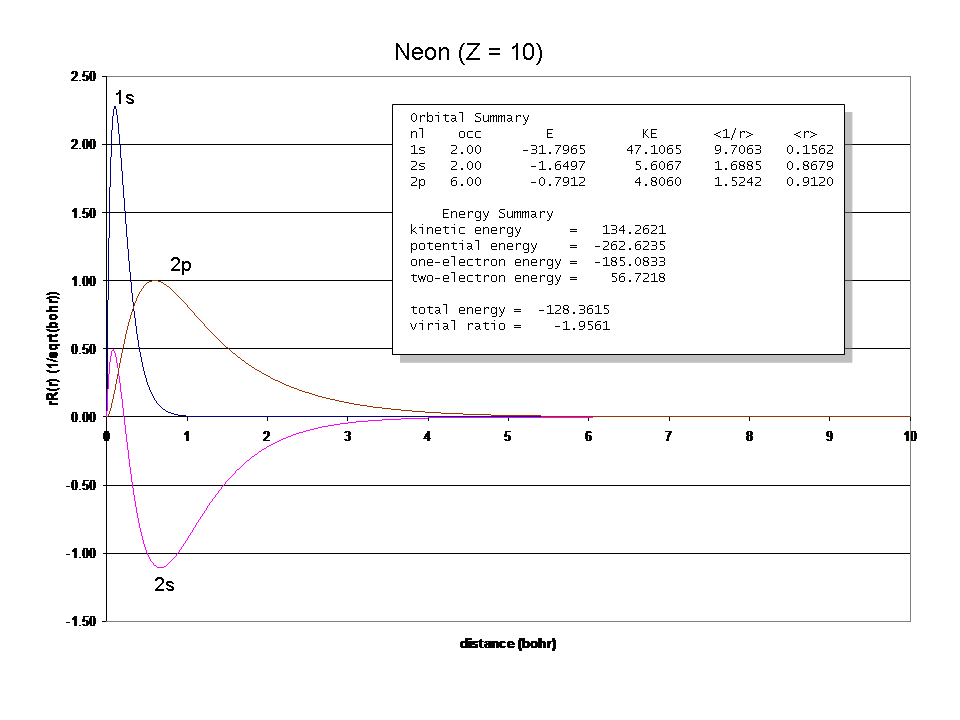
\includegraphics[scale=0.33]{Images/Slide3.png} & 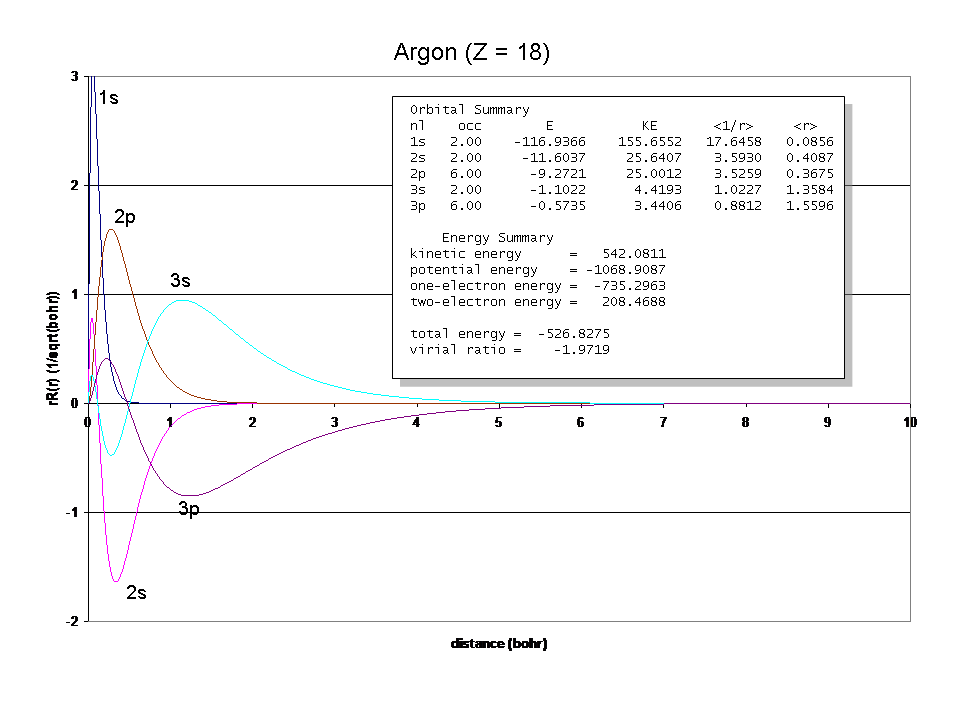
\includegraphics[scale=0.33]{Images/Slide4.png} \\
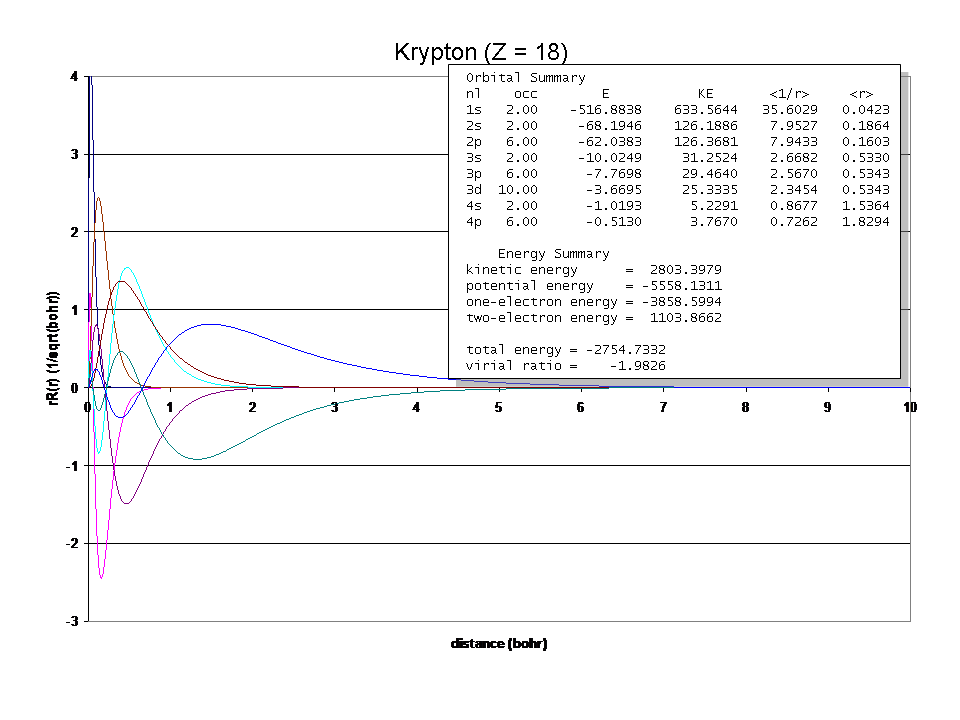
\includegraphics[scale=0.33]{Images/Slide5.png} & 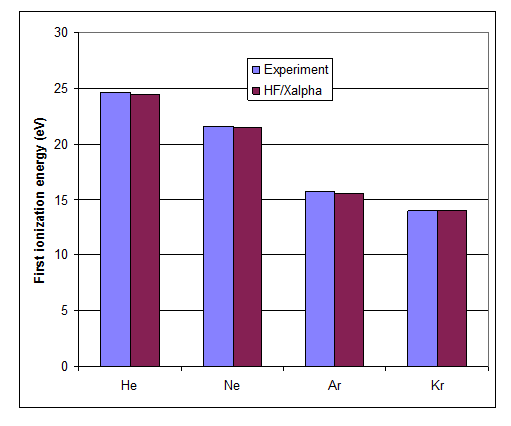
\includegraphics[scale=0.5]{Images/Slide6.png} 
\end{tabular}
\end{table}

\subsection{Lecture 13: Molecular orbital theory of molecules}
\label{sec:orge05e143}
\subsubsection{Clamped nucleus (``Born-Oppenheimer'') approximation}
\label{sec:org5e3ec2b}
\begin{enumerate}
\item Write one-electron equations parametrically in terms of positions of  all atoms
\begin{eqnarray}
\hat h & = & -\frac{\hbar^2}{2m_e}\nabla^2-\sum_\alpha \frac{Z_\alpha
    e^2}{4\pi\epsilon_0}\frac{1}{|{\bf r}-{\bf R}_\alpha|} \\
\hat f\psi & = & \left\{\hat h + \hat v_\mathrm{Coul}[\psi_i] + \hat
      v_\mathrm{ex}[\psi_i]+\hat v_\mathrm{corr}[\psi_i] \right\}\psi=\epsilon\psi
\end{eqnarray}
\item Solve as for atoms, using some model for electron-electron interactions
\item Potential energy surface (PES)
\[ E({\bf R}_\alpha, {\bf
            R}_\beta,...)=E_\mathrm{elec}+\frac{e^2}{4\pi\epsilon_0}\sum_\alpha\sum_{\beta>\alpha}\frac{Z_\alpha
            Z_\beta}{|{\bf R}_\alpha-{\bf R}_\beta|} \]
\end{enumerate}
\subsubsection{H\(_2\) molecule as perturbation on two H atoms brought from infinite distance}
\label{sec:org95ecfdb}
\begin{enumerate}
\item ``Bonding'' orbital, \(\sigma_g({\bf r}) = 1{\rm s_A}+1{\rm s_B}\)
\item ``Anti-bonding'' orbital, \(\sigma_u({\bf r}) = 1{\rm s_A}-1{\rm s_B}\)
\item Interaction scales with ``overlap'' \(S = \langle 1{\rm s_A} | 1{\rm
            s_B} \rangle\)
\item Normalize
\begin{displaymath}
\sigma_g = \frac{1}{\sqrt{2(1-S)}}\left ( 1{\rm s_A}+1{\rm s_B} \right)     \quad\quad
\sigma_u = \frac{1}{\sqrt{2(1+S)}}\left ( 1{\rm s_A}-1{\rm s_B} \right)
\end{displaymath}
\item Energy expectation value
\begin{eqnarray*}
\epsilon_g = \langle \sigma_g | \hat{f} | \sigma_g \rangle & = & \frac{1}{2(1+S)} \left \{ \langle 1{\rm s_A} | \hat{f} | 1{\rm s_A} \rangle +  \langle 1{\rm s_B} | \hat{f} | 1{\rm s_B} \rangle + 2 \langle 1{\rm s_A} | \hat{f} |1{\rm s_B} \rangle \right \}\\
& = & \frac{1}{1+S} \left ( F_{\rm AA} + F_{\rm AB} \right ) \\
\epsilon_u = \langle \sigma_u | \hat{f} | \sigma_u \rangle & = & \frac{1}{2(1+S)} \left \{ \langle 1{\rm s_A} | \hat{f} | 1{\rm s_A} \rangle + \langle 1{\rm s_B} | \hat{f} | 1{\rm s_B} \rangle - 2 \langle 1{\rm s_A} | \hat{f} | 1{\rm s_B} \rangle\right \}\\
& = & \frac{1}{1-S} \left ( F_{\rm AA} - F_{\rm AB} \right )
\end{eqnarray*}
\item Matrix elements
\begin{eqnarray*}
  F_{\rm AA}=F_{\rm BB}\approx \epsilon_{1\mathrm{s}}=\alpha \\
  F_{\rm AB}=F_{\rm BA}=\beta \\
  \alpha < \beta < 0\ \ \mathrm{typically}
\end{eqnarray*}
\begin{center}
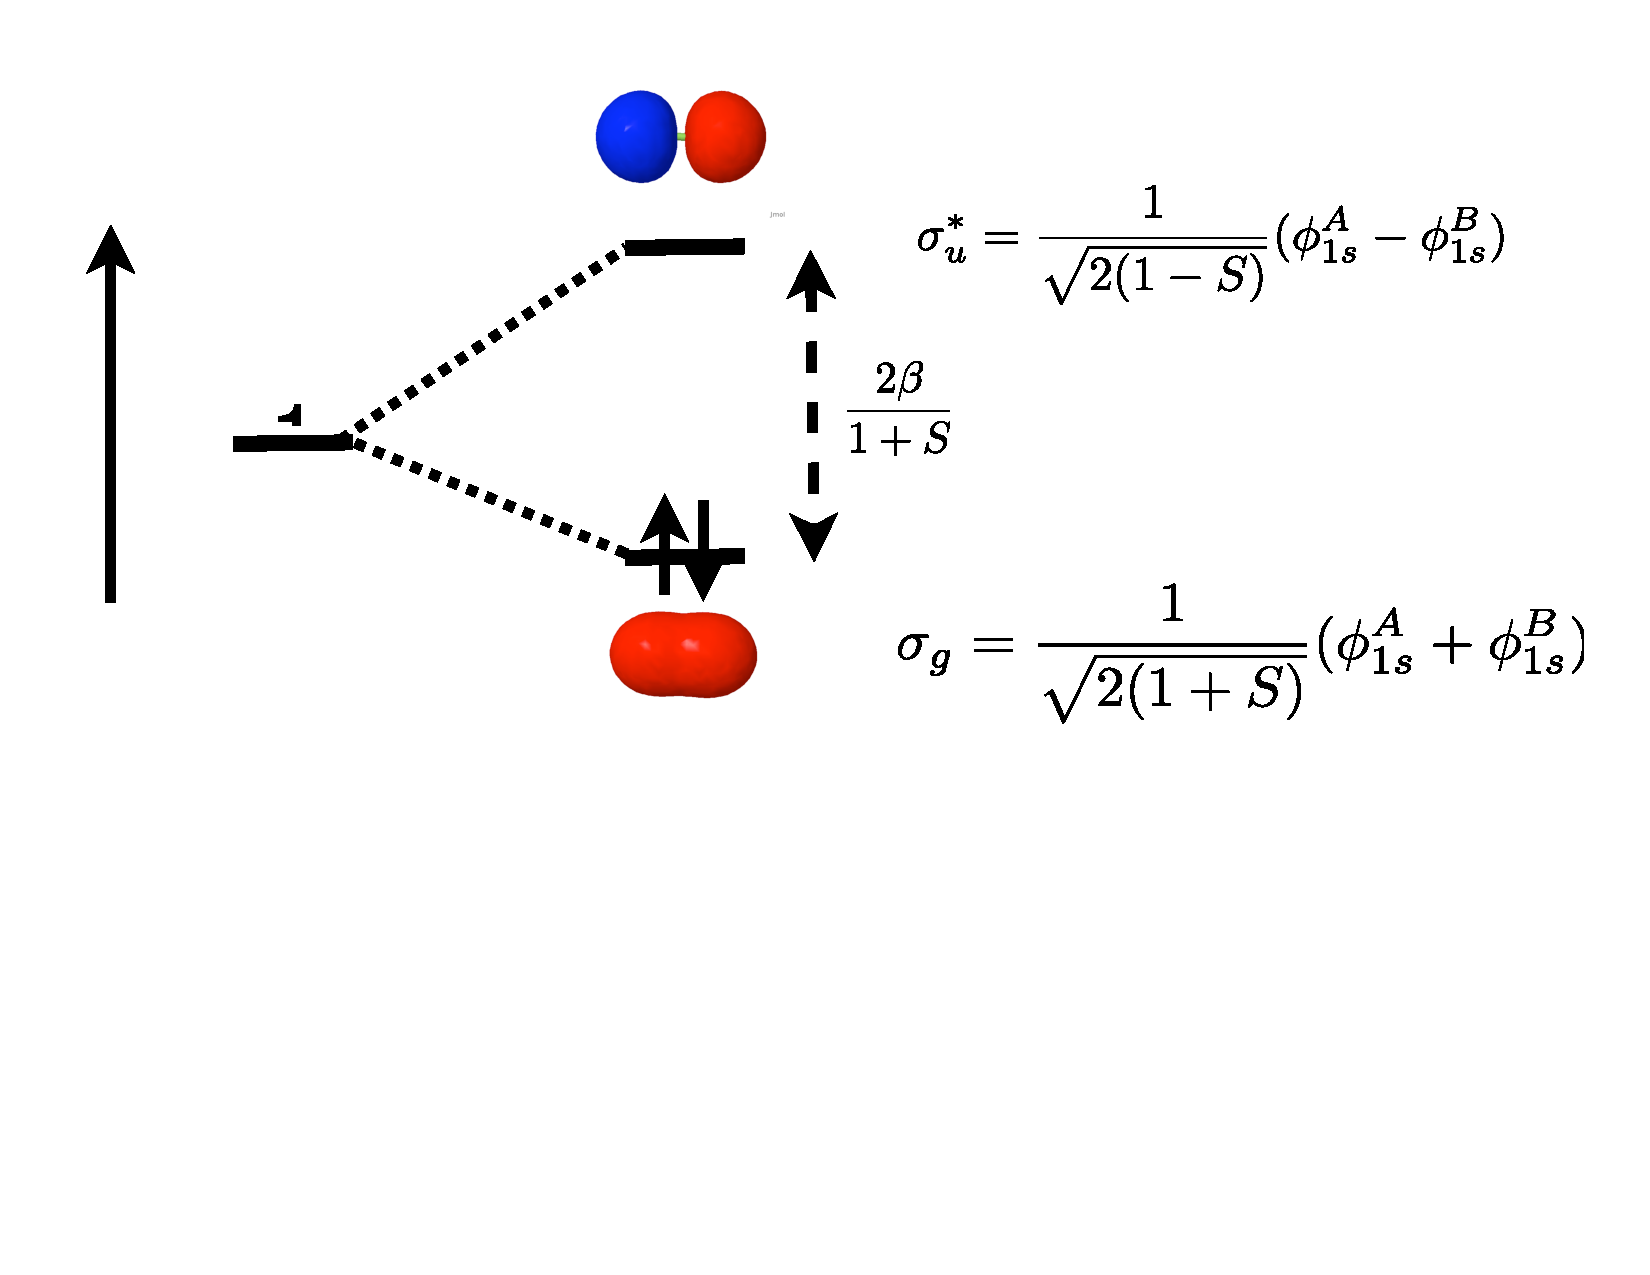
\includegraphics[scale=0.5]{./Images/H2-MO}       
\end{center}
\item From Taylor expansion get picture of atomic orbitals destabilized by electron repulsion \(\beta S\) and split by interaction \(\beta\)
\begin{eqnarray*}
  \epsilon_+\approx \alpha-\beta S + \beta \\
  \epsilon_-\approx \alpha - \beta S - \beta
\end{eqnarray*}
\item Makes clear that bonding stabilization \(<\) anti-bonding destabilization
\item Ground configuration \(=\sigma_g^2\)
\item Bond order = \(\frac{1}{2}(n-n^*)\)
\end{enumerate}
\subsubsection{Secular equations}
\label{sec:orgdf34908}
\begin{enumerate}
\item Expand molecular orbitals in ``basis'' of atomic-like orbitals
\begin{equation}
  \psi_\mathrm{MO}=\sum_a c_a\phi_a({\bf r})
\end{equation}
\item Problem reduces to finding set of \(c_a\) that give best molecular orbitals (MOs)
\item Substituting into Fock equation and integrating yields set of linear equations for the \(c_a\) for each MO
  \begin{displaymath}
    \left ( \begin{array}{ccc}
      F_{11}-\epsilon S_{11} & F_{12}-\epsilon S_{12} & \ldots \\
      F_{21}-\epsilon S_{21} & F_{22}-\epsilon S_{22} & \ldots \\
      \vdots & \vdots & \vdots
    \end{array} \right ) \left (
    \begin{array}{c}
      c_1 \\
      c_2 \\
      \vdots
    \end{array} \right ) = 0
\end{displaymath}
\begin{enumerate}
\item \(F_{ij} = F_{ji} = \langle \phi_i | \hat f | \phi_j \rangle\) are Fock
``matrix elements''
\item \(S_{ij} = S_{ji} = \langle \phi_i | \phi_j \rangle\) are overlaps
\item Typically basis functions normalized such that \(S_{ii} = 1\)
\item \(\epsilon\) are molecular orbital energies (to be solved for, as many as there are equations)
\end{enumerate}
\item From linear algebra, only possible solutions are those that make the determinant vanish
  \begin{displaymath}
    \left | \begin{array}{ccc}
      F_{11}-\epsilon S_{11} & F_{12}-\epsilon S_{12} & \ldots \\
      F_{21}-\epsilon S_{21} & F_{22}-\epsilon S_{22} & \ldots \\
      \vdots & \vdots & \vdots
    \end{array} \right | = 0
\end{displaymath}
\item Solve for \(\epsilon\)s and back-substitute to find correspond \(c_i\)s
\end{enumerate}
\subsubsection{H\(_2\) example, again}
\label{sec:orgce5fb5b}
\begin{enumerate}
\item Set-up and solve secular matrix
\begin{displaymath}
 \left | \begin{array}{cc}
     \alpha-\epsilon & \beta-\epsilon S \\
     \beta - \epsilon S & \alpha-\epsilon
     \end{array} \right | = 0
\end{displaymath}
\begin{eqnarray*}
  \epsilon_+=\frac{\alpha+\beta}{1+S},\ \ c_1=c_2=\frac{1}{\sqrt{2(1+S)}} \\
  \epsilon_-=\frac{\alpha-\beta}{1-S},\ \ c_1=-c_2=\frac{1}{\sqrt{2(1-S)}} \\
\end{eqnarray*}
\end{enumerate}
\subsubsection{Qualitative solutions of secular equations}
\label{sec:orgb1274a9}
\begin{enumerate}
\item Lot's of insight into chemical bonding can be obtained from approximate solutions to secular equations, basis of ``molecular orbital theory''
\item Two general assumptions
\begin{enumerate}
\item Diagonal Fock elements are approximately equal to energies of corresponding atomic orbitals: \(F_{ii} \approx \epsilon_{i,\mathrm{ao}}\)
\item Off-diagonal elements proportional to overlap and inversely proportional to energy difference:
\begin{displaymath}
  F_{ij} \propto \frac{S_{ij}}{\epsilon_{i,\mathrm{ao}}-\epsilon_{j,\mathrm{ao}}}
\end{displaymath}
\item (Often) set differential overlap \(S_{ij}=0\)
\end{enumerate}
\end{enumerate}

\subsubsection{Heteronuclear diatomic: LiH, HF, BH example}
\label{sec:org0d45053}
\begin{enumerate}
\item Only AOs of appropriate symmetry, overlap, and energy match can combine to form MOs
\begin{eqnarray*}
  \epsilon_+\approx \alpha_1- \beta S  - \beta^2/|\alpha_1-\alpha_2| \\
  \epsilon_-\approx \alpha_2 - \beta S + \beta^2/|\alpha_1-\alpha_2|
\end{eqnarray*}
\item LiH: H 1s + Li 2s, bond polarized towards H
\item HF: H 1s + F 2p, bond polarized towards F, lots of non-bonding orbitals
\item BH: H 1s, B 2s and 2p\(_z \rightarrow\) bonding, non-bonding, anti-bonding orbitals
\end{enumerate}
\subsubsection{Homonuclear diatomic: O\(_2\)}
\label{sec:org95a8191}
\begin{enumerate}
\item Assign aos, 1s, 2s, 2p for each atom (10 total)
\item In principle, solve \(10\times 10\) secular matrix
\item In practice, matrix elements rules mean only a few off-diagonal elements survive
\begin{enumerate}
\item 1s + 1s do nothing
\item 2s + 2s form \(\sigma\) bond and anti-bond
\item 2p\(_z\) + 2p\(_z\) form second bond and anti-bond
\item 2p\(_{x,y}\) + 2p\(_{x,y}\) form degenerate \(\pi\) bonds and anti-bonds
\item O\(_2\) is a triplet, consistent with experiment!
\end{enumerate}
\end{enumerate}
\subsubsection{The H\"{u}ckel/tight binding model: \href{http://resolver.caltech.edu/CaltechBOOK:1961.001}{Roberts, Notes on Molecular Orbital Theory}}
\label{sec:orgcc277d9}
\begin{enumerate}
\item \(F_{ii}=\alpha, S_{ij}=\delta_{ij}, F_{ij}=\beta\) iff \(i\) adjacent to \(j\)
\item Ethylene example
\item Butadiene example
\item Benzene example
\item Infinite chain example
\end{enumerate}

\begin{minted}[frame=lines,fontsize=\scriptsize,linenos]{python}
from sympy import *
init_printing(use_unicode=True)

print('6. Cyclobutadiene example\n')
alpha,beta = symbols('alpha beta')

M = Matrix([[alpha, beta, 0 , beta],[beta, alpha, beta, 0],[0,beta,alpha,beta],[beta,0,beta,alpha]])

print(M)
# M = Matrix([[alpha,beta],[beta,alpha]])

eigs  = M.eigenvects()

print("\nEnergy state, degeneracy\n")
for state in [0, 1, 2]:
    print('{0}    {1}\n'.format(eigs[state][0],eigs[state][1]))

#print("\nEigenvectors")
#for state in [0, 1, 2]:
#    print(eigs[state][2])

\end{minted}

\begin{enumerate}
\item Cyclobutadiene example
\end{enumerate}

Matrix([[alpha, beta, 0, beta], [beta, alpha, beta, 0], [0, beta, alpha, beta], [beta, 0, beta, alpha]])

Energy state, degeneracy

alpha    2

alpha - 2*beta    1

alpha + 2*beta    1

\subsubsection{Band structure of solids}
\label{sec:org435e708}
\begin{enumerate}
\item Discrete molecular orbitals transform into continuous bands
\item Results in rich range of physical and chemical properties
\end{enumerate}

\begin{center}
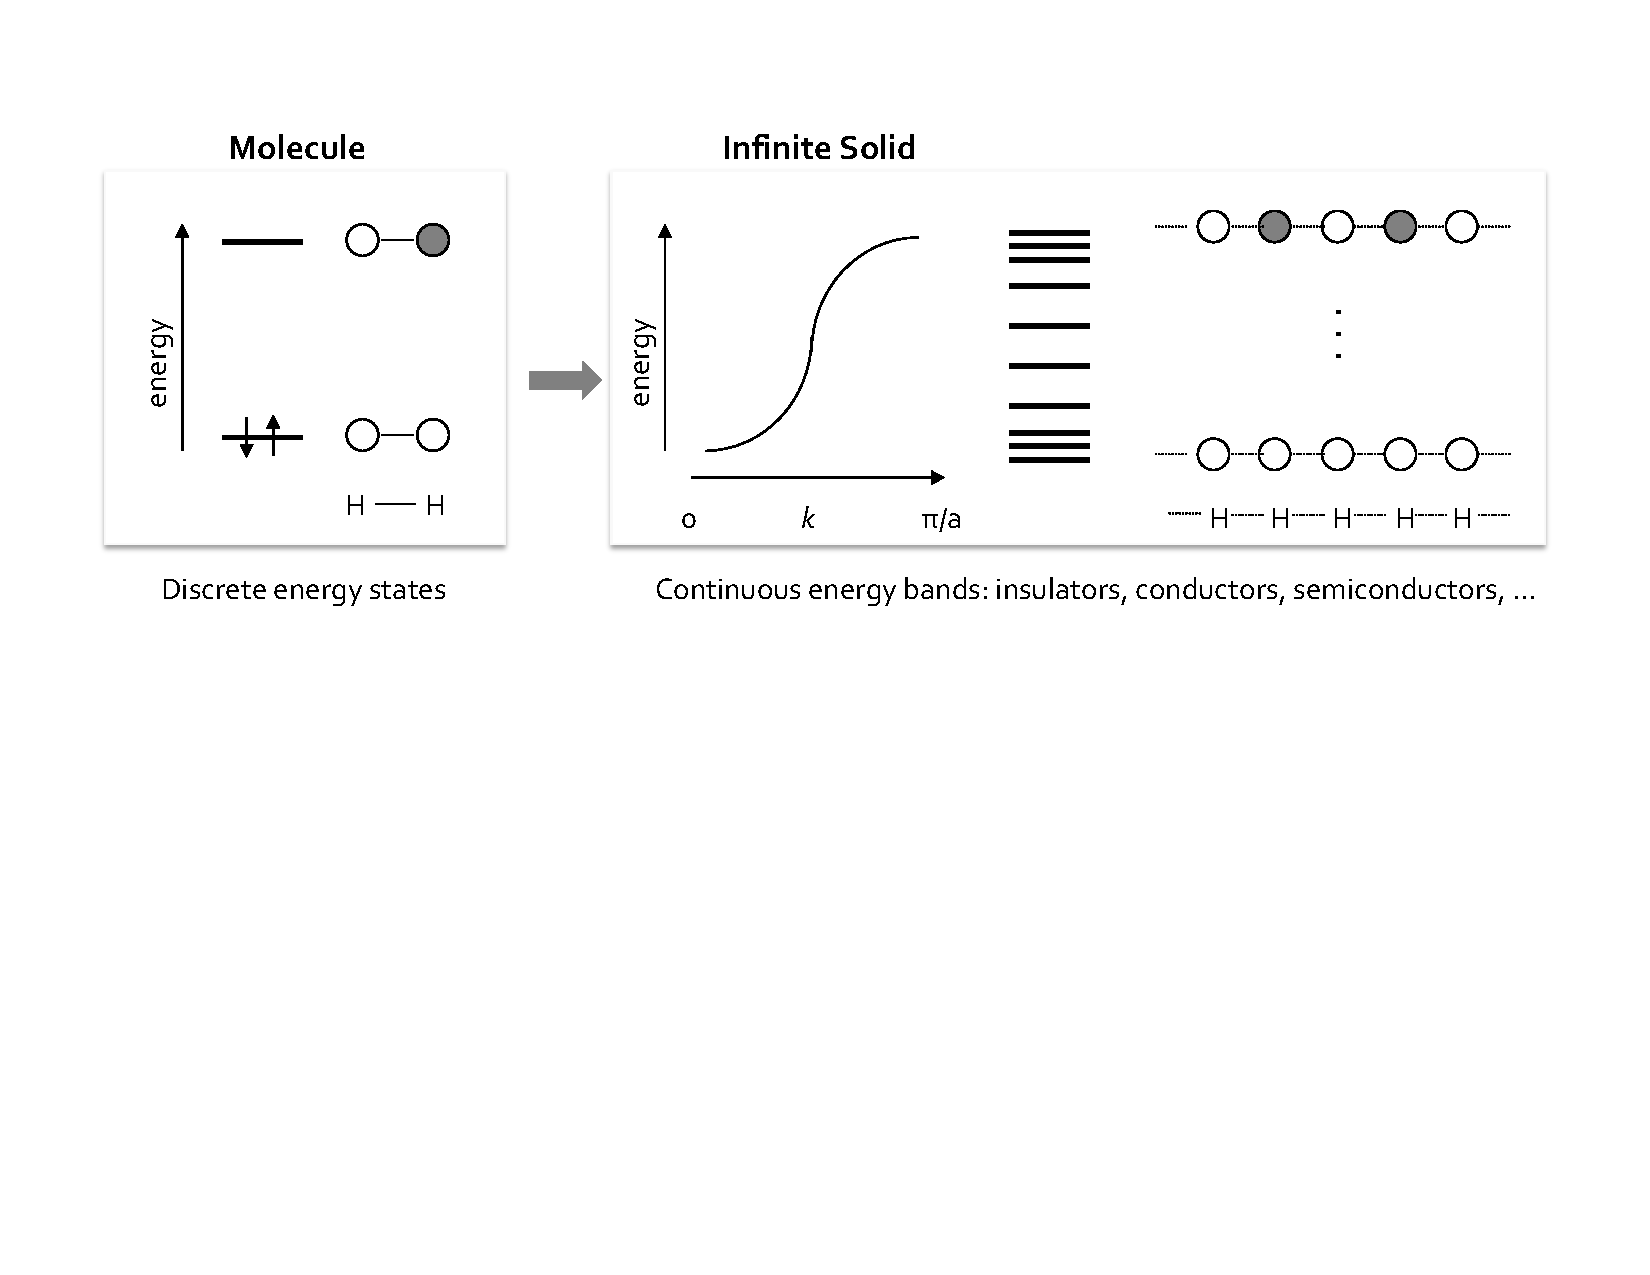
\includegraphics[width=0.9\textwidth]{./Images/band.pdf}
\end{center}

\subsection{Lecture 14: Computational chemistry}
\label{sec:orgde00606}
\subsubsection{Numerical solvers of Schr\"{o}dinger equation for molecules readily available today}
\label{sec:orgc0fc71a}
\subsubsection{Have to specify:}
\label{sec:org6f6e381}
\begin{enumerate}
\item Identity of atoms
\item Positions of atoms (distances, angles, \(\ldots\))
\item (spin multiplicity)
\item exact theoretical model (how are Coulomb, exchange, and correlation described?)
\begin{enumerate}
\item Hartree, Hartree-Fock, DFT (various flavors), \(\ldots\)
\end{enumerate}

\item basis set to express wavefunctions in terms of
\item initial guess of wavefunction coefficients (often guessed for you)
\end{enumerate}
\subsubsection{Secular equations solved iteratively until input coefficients = output coefficients}
\label{sec:orgc9a35fd}
\begin{enumerate}
\item ``self-consistent field''
\item Output
\begin{enumerate}
\item energies of molecular orbitals
\item occupancies of molecular orbitals
\item coefficients describing molecular orbitals
\item total electron wavefunction, total electron density, dipole moment, \(\ldots\)
\item total molecular energy
\item derivatives (``gradients'') of total energy w.r.t. atom positions
\end{enumerate}
\item Plot total energy vs internal coordinates: potential energy surface (PES)
\item Search iteratively for minimum point on PES (by hand or using gradient-driven search): equilibrium geometry
\item Find second derivative of energy at minimum point on PES: harmonic vibrational frequency
\item Find energy at minimum relative to atoms (or other molecules): reaction energy
\end{enumerate}
\subsubsection{H\(_2\) example}
\label{sec:orga91725c}
\begin{center}
  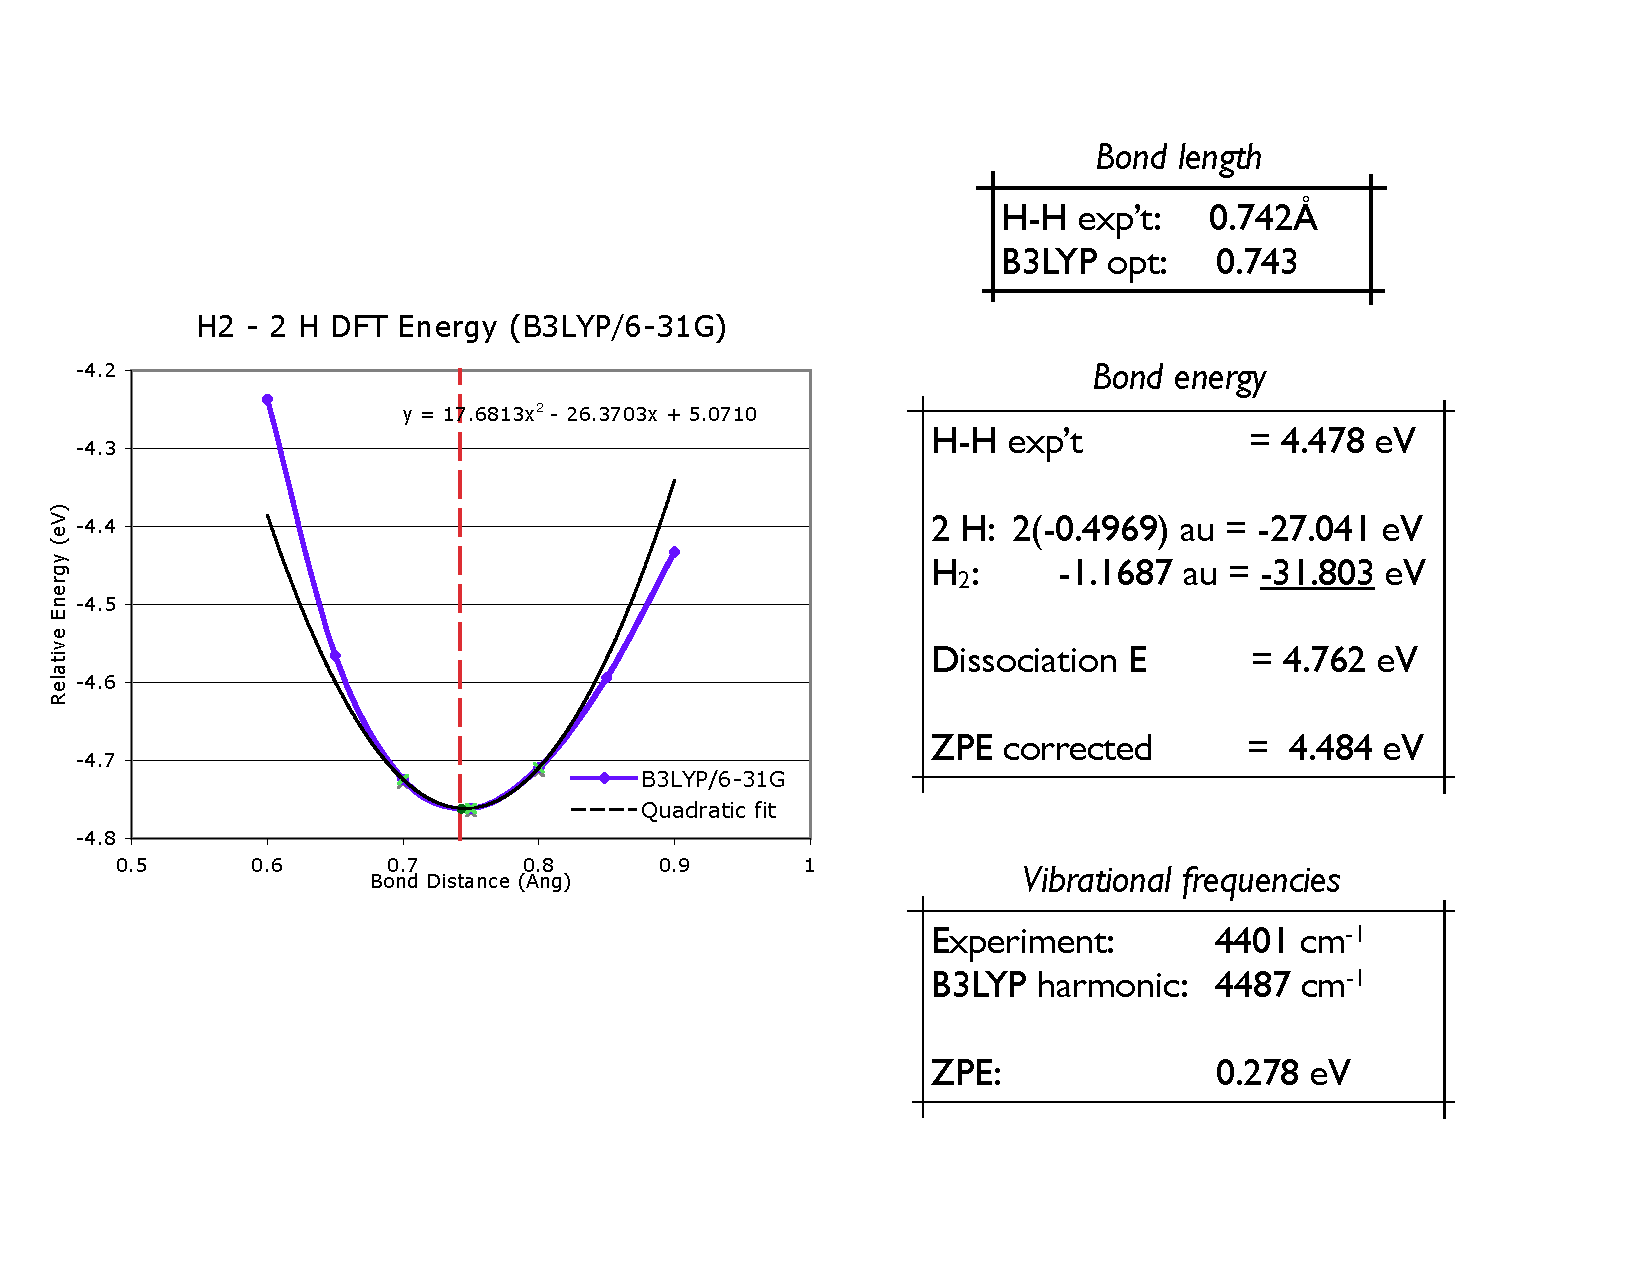
\includegraphics[scale=0.6]{Images/H2-PES}
\end{center}
\subsubsection{Polyatomic molecules}
\label{sec:org211f0e9}
\begin{enumerate}
\item Gradient-driven optimizations, \(3n-6\) degrees of freedom
\item Hessian matrix for frequencies
\end{enumerate}

\subsection{Lecture 15: Electronic spectroscopy}
\label{sec:orga646246}
\subsection{Lecture 16: Electronic and magnetic properties}
\label{sec:org4979585}

\section{Statistical Mechanics: The Bridge from the Tiny to the Many}
\label{sec:org7fa5cb4}

\subsection{Lecture 17: Statistical mechanics}
\label{sec:org29509ac}
\subsubsection{Need machinary to average QM information over macroscopic systems}
\label{sec:orge618c21}
\subsubsection{Equal \emph{a priori} probabilities}
\label{sec:org35cc24e}
\subsubsection{Two-state model}
\label{sec:org53a0ecb}
\begin{enumerate}
\item Box of particles, each of which can have energy 0 or \(\epsilon\)
\item Thermodynamic state defined by number of elements \(N\), and number of quanta \(q\), \(U=q\epsilon\)
\item Degeneracy of given \(N\) and \(q\) given by binomial distribution:
\begin{displaymath}
  \Omega=\frac{N!}{q!(N-q)!}
\end{displaymath}
\item Allow energy to flow between two such systems
\begin{enumerate}
\item Energy of a closed system is conserved (first law!)
\item Degeneracy of total system is always \(\geq\) degeneracy of the starting parts!
\item Boltzmann's tombstone, \(S = k_B \ln \Omega\)
\item Clausius: entropy of the universe seeks a maximum!  Second Law\ldots{}
\end{enumerate}
\end{enumerate}

\subsubsection{Energy flow/thermal equilibrium between two large systems}
\label{sec:orge34a4a7}
\begin{enumerate}
\item Each subsystem has energy \(U_i\) and degeneracy \(\Omega_i(U_i)\)
\item Bring in thermal contact, \(U=U_1+U_2\), \(\Omega=\Omega_1(U_1)\Omega_2(U_2)\)
\item If systems are very large, one combination of \(U_1\), \(U_2\) and \(\Omega\) will be much more probably than all others
\item What value of \(U_1\) and \(U_2=U-U_1\) maximizes \(\Omega\)?
       \begin{displaymath}
\left ( \frac{\partial \ln \Omega_1}{\partial U_1} \right )_N = \left ( \frac{\partial \ln \Omega_2}{\partial U_2} \right )_N
       \end{displaymath}
       \begin{displaymath}
\left ( \frac{\partial S_1}{\partial U_1} \right )_N = \left ( \frac{\partial S_2}{\partial U_2} \right )_N
       \end{displaymath}
\item Thermal equilibrium is determined by equal \textbf{temperature}!
\begin{displaymath}
    \frac{1}{T}=\left ( \frac{\partial S}{\partial U} \right )_N
  \end{displaymath}
\item When the temperatures of the two subsystems are equal, the entropy of the combined system is maximized!
\item (Same arguments lead to requirement that equal pressures (\(P_i\)) and equal chemical potentials (\(\mu_i\)) maximize entropy when volumes or particles are exchanged)
\end{enumerate}

\subsubsection{Two-state model in limit of large \(N\)}
\label{sec:org4cad1a5}
\begin{enumerate}
\item Large \(N\) and Stirling's approximation
\item Fundamental thermodynamic equation of two-state system:
\begin{displaymath}
  S(U)=-k_B \left ( x \ln x + (1-x) \ln (1-x) \right ), \mathrm{where}\
  x = q/N = U/N\epsilon
\end{displaymath}
\item Temperature is derivative of entropy wrt energy yields
\begin{displaymath}
  U(T) = \frac{N\epsilon}{1+e^{\epsilon/k_BT}}
\end{displaymath}
\item \(T \rightarrow 0, U \rightarrow 0, S \rightarrow 0\), minimum disorder
\item \(T \rightarrow \infty, U \rightarrow N\epsilon/2, S \rightarrow k_B \ln 2\), maximum disorder
\item Differentiate again to get heat capacity
\end{enumerate}
\subsubsection{Example of microcanonical (``\(NVE\)'') ensemble}
\label{sec:org2f428b8}
\begin{enumerate}
\item Direct evaluation of \(S(U)\) is generally intractable, so seek simpler approach
\end{enumerate}
\subsection{Lecture 18: Canonical (\(NVT\)) ensemble}
\label{sec:org9a33f20}
\subsubsection{Partition function}
\label{sec:org10a3289}
\begin{enumerate}
\item Imagine a system brought into thermal equilibrium with a much larger ``reservoir'' of constant \(T\), such that the aggregate has a total energy \(U\)
\item Degeneracy of a given system microstate \(j\) with energy \(U_j\) is \(\Omega_{res}(U-U_j)\)
\begin{eqnarray*}
  T = \frac{dU_{res}}{k_Bd\ln\Omega_{res}} \\
  \Omega_{res}(U-U_j) \propto e^{-U_j/k_B T}
\end{eqnarray*}
\item Probability for system to be in a microstate with energy \(U_j\) given by Boltzmann distribution!
\begin{displaymath}
  P(U_j) \propto e^{-U_j/k_B T} = e^{-U_j \beta}
\end{displaymath}
\item Partition function ``normalizes'' distribution, \(Q(T,V) = \sum_j e^{-U_j \beta}\)
\end{enumerate}

\begin{enumerate}
\item \textbf{Partition function counts the number of states accessible to a system at a given \(T\) and \(V\)}
\end{enumerate}
\subsubsection{Energy factoring (sidebar)}
\label{sec:org1720e75}
\begin{enumerate}
\item If system is large, how to determine it's energy states \(U_j\)?  There would be many, many of them!
\item One simplification is if we can write energy as sum of energies of individual elements (atoms, molecules) of system:
\begin{align}
  U_j&=\epsilon_j(1)+\epsilon_j(2) + ... + \epsilon_j(N) \\
  Q(N,V,T) &= \sum_j e^{-U_j\beta} \\
  &=\sum_je^{-(\epsilon_j(1)+\epsilon_j(2) + ... + \epsilon_j(N))\beta}
\end{align}
\item \emph{If} molecules/elements of system can be distinguished from each
other (like atoms in a fixed lattice), expression can be factored:
   \begin{align}
     Q(N,V,T)&=\left ( \sum_j e^{-\epsilon_j(1)\beta}\right )\cdots \left ( \sum_j
       e^{-\epsilon_j(N)\beta}\right ) \\
   &= q(1)\cdots q(N) \\
   \text{Assuming all the elements are the same:}\\
   &= q^N \\
  q&=\sum_j e^{-\epsilon_j \beta}: \mathrm{molecular\ partition\ function}
\end{align}
\item \emph{If not} distinguishable (like molecules in a liquid or gas, or electrons in a solid), problem is difficult, because identical
arrangements of energy amongst elements should only be counted once.
\item Approximate solution, good almost all the time:
\begin{equation}
  Q(N,V,T)=q^N/N!
\end{equation}
\item Sidebar: ``Correct'' factoring depends on whether individual elements are fermions or bosons, leads to funny things like superconductivity and superfluidity.
\end{enumerate}

\subsubsection{Distinguishable vs. indistinguishable particles}
\label{sec:org6abd08f}
\begin{enumerate}
\item \(q(V,T)\) counts states available to a single element of a system, like a molecule in a gas or in a solid
\item Distinguishable (e.g., in a solid): \(Q(N,V,T) = q(V,T)^N\)
\item Indistinguishable (e.g., a gas): \(Q(N,V,T)\approx q(V,T)^N/N!\)
\end{enumerate}

\subsubsection{Two-state system again}
\label{sec:org407a134}
\begin{enumerate}
\item Partition function, \(q(T)=1+e^{-\epsilon\beta}\)
\item State probabilities
\item Internal energy \(U(T)\)
\begin{equation}
  U(T)=-N \left ( \frac{\partial \ln(1+e^{-\epsilon\beta})}{\partial\beta}
  \right)=\frac{N\epsilon e^{-\epsilon\beta}}{1+e^{-\epsilon\beta}}
\end{equation}
\item Heat capacity \(C_v\)
\begin{enumerate}
\item Minimum when change in states with \(T\) is small
\item Maximize when chagne in states with \(T\) is large
\end{enumerate}
\item Helmholtz energy, \(A= -\ln q/\beta\), decreasing function of \(T\)
\item Entropy
\end{enumerate}

\begin{table}
   \caption{Two-state system thermodynamics}
\begin{tabular}{cc}
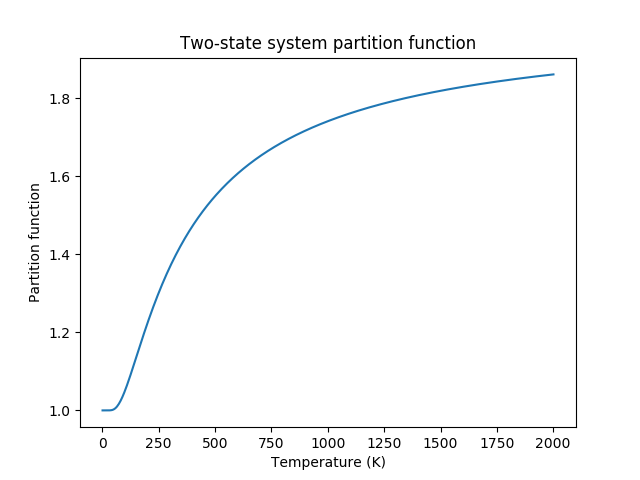
\includegraphics[scale=0.5]{Images/2state-partition.png} & 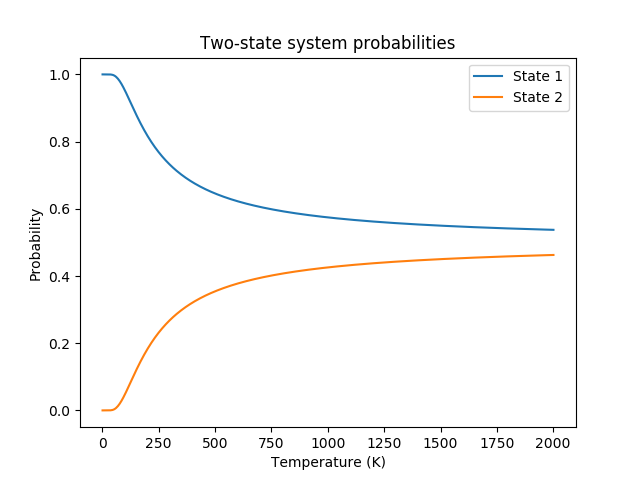
\includegraphics[scale=0.5]{Images/2state-probability.png} \\
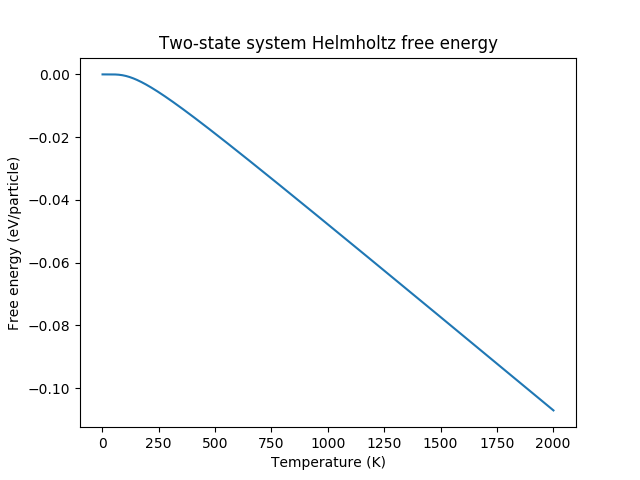
\includegraphics[scale=0.5]{Images/2state-helmholtz.png} & 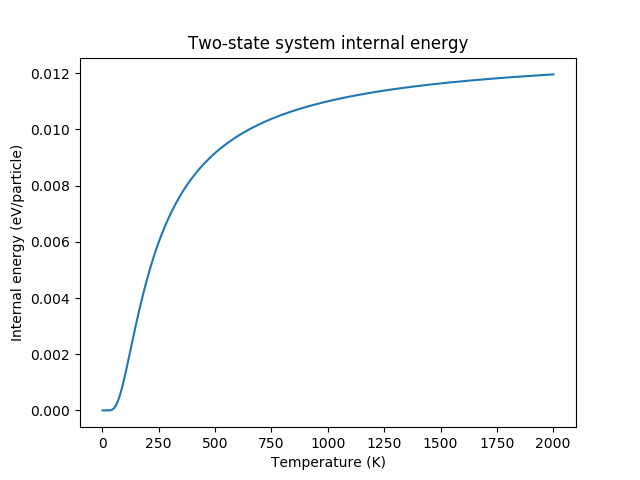
\includegraphics[scale=0.5]{Images/2state-internal.png} \\
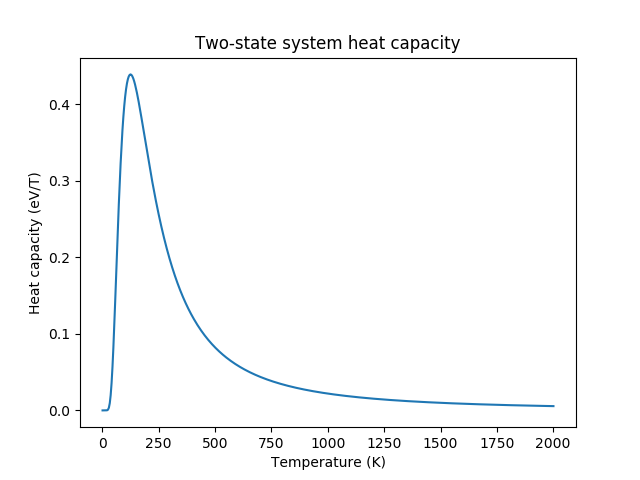
\includegraphics[scale=0.5]{Images/2state-heatcapacity.png} & 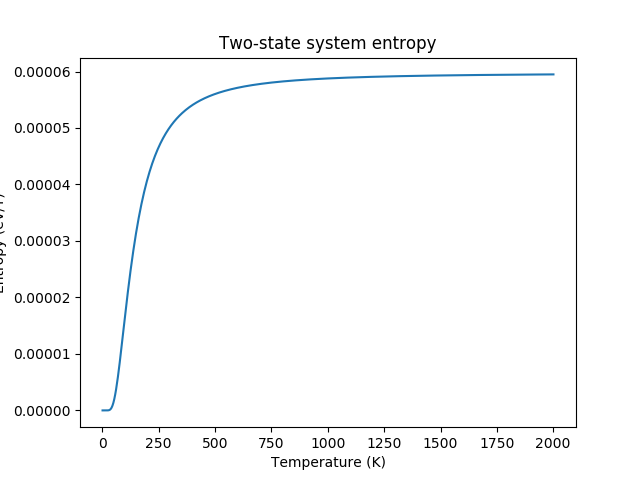
\includegraphics[scale=0.5]{Images/2state-entropy.png}
\end{tabular}
\end{table}

\subsubsection{Thermodynamic functions in canonical ensemble}
\label{sec:org43f52a2}

\begin{table}\small
  \begin{center}
    \caption{Equations of the Canoncial ($NVT$) Ensemble}
    \label{Canonical}
    \begin{tabular}[h]{lccc}
      \hline
$\beta=1/k_BT$ & {\bf Full Ensemble} & {\bf Distinguishable particles} & {\bf Indistinguishable
particles} \\
               &               & (e.g. atoms in a lattice) & (e.g. molecules in
               a fluid) \\
\hline
Single particle & & & \\partition function& & $\displaystyle q(V,T) = \sum_i
e^{-\epsilon_i\beta} $& $\displaystyle q(V,T) = \sum_i e^{-\epsilon_i\beta} $ \\
Full partition & & & \\function & $\displaystyle Q(N,V,T) = \sum_j e^{-U_j\beta} $ &
$\displaystyle Q = q(V,T)^N $ & $\displaystyle Q = q(V,T)^N/N! $ \\
Log partition &  $\ln Q$ & $N\log q$ & $ N\ln q - \ln N! $\\
function & & & $\approx N(\ln Q - \ln N +1)$ \\ & & & \\
Helmholtz energy & $\displaystyle -\frac{\ln Q}{\beta}$ & $\displaystyle
-\frac{N\ln q}{\beta}$ & $\displaystyle -\frac{N}{\beta}\left (\ln\frac{q}{N} +
  1 \right ) $ \\
($A=U-TS$) & & & \\ & & &  \\
Internal energy ($U$)& $\displaystyle -\left (\frac{\partial\ln
    Q}{\partial\beta}\right )_{NV}$ & $\displaystyle -N\left (\frac{\partial\ln
    q}{\partial\beta}\right )_{V}$ &  $\displaystyle -N\left (\frac{\partial\ln
    q}{\partial\beta}\right )_{V}$ \\ & & & \\
Pressure ($P$) & $\displaystyle  \frac{1}{\beta}\left (\frac{\partial\ln
    Q}{\partial V}\right )_{N\beta}$ & $\displaystyle \frac{N}{\beta}\left (\frac{\partial\ln
    q}{\partial V}\right )_{\beta}$ &  $\displaystyle \frac{N}{\beta}\left (\frac{\partial\ln
    q}{\partial V}\right )_{\beta}$ \\ & & & \\

Entropy ($S/k_B$) & $ \beta U + \ln Q$ & $\beta U + N \ln q$ & $\beta U +
N\left ( \ln(q/N) + 1\right )$ \\ & & & \\
Chemical potential ($\mu$) & $\displaystyle -\frac{1}{\beta}\left ( \frac{\partial \ln
    Q}{\partial N}\right )_{VT} $& $\displaystyle -\frac{\ln q}{\beta}$ & $\displaystyle
-\frac{\ln (q/N)}{\beta}$ \\ & & & \\
\hline
    \end{tabular}
{\bf NOTE!} All energies are referenced to their values at 0~K.  Enthalpy $H=U+PV$, Gibb's
Energy $G=A+PV$.
  \end{center}
\end{table}

\subsection{Lecture 19: Molecular Partition Functions}
\label{sec:org02fa928}
\subsubsection{Ideal gas of molecules}
\label{sec:org584ba42}
\begin{displaymath}
  Q_{ig}(N,V,T) = \frac{(q_\mathrm{trans}q_\mathrm{rot}q_\mathrm{vib})^N}{N!}
\end{displaymath}

\subsubsection{Particle-in-a-box (translational states of a gas)}
\label{sec:orgce4f65b}
\begin{enumerate}
\item Energy states \(\epsilon_n=n^2\epsilon_0, n=1,2, \ldots\), \(\epsilon_0\) tiny for macroscopic \(V\)
\item \(\Theta_\mathrm{trans} = \epsilon_0/k_B\) translational temperature
\item \(\Theta_\mathrm{trans} << T \rightarrow\) many states contribute to \(q_\mathrm{trans}\rightarrow\) integral approximation
\begin{eqnarray*}
  q_\mathrm{trans,1D} \approx \int_0^\infty e^{-x^2\beta\epsilon_0}dx =
  L/\Lambda \\
  \Lambda = \left ( \frac{h^2\beta}{2\pi m} \right )^{1/2}\
  \mathrm{thermal\ wavelength} \\
  q_\mathrm{trans,3D} = V/\Lambda^3
\end{eqnarray*}
\item Internal energy
\item Heat capacity
\item Equation of state (!)
\item Entropy: Sackur-Tetrode equation
\end{enumerate}

\subsubsection{Rigid rotor (rotational states of a gas)}
\label{sec:orga2196c6}
\begin{enumerate}
\item recall energy states and degeneracies of rigid rotor
\item \(\Theta_\mathrm{rot} = \hbar^2/2 I k_B\)
\item ``High'' T \(q_\mathrm{rot}(T) \approx \sigma \Theta_\mathrm{rot}/T\)
\end{enumerate}
\subsubsection{Harmonic oscillator (vibrational states of a gas)}
\label{sec:orge72e6f4}
\begin{enumerate}
\item \(\Theta_\mathrm{vib}=h\nu/k_B\)
\end{enumerate}

\subsubsection{Electronic partition functions \(\rightarrow\) spin multiplicity}
\label{sec:org8b0d9ac}

\subsubsection{Many-particle molecule}
\label{sec:org1eebfcd}
\begin{enumerate}
\item partition function is a product of all degrees of freedom
\begin{displaymath}
q(T,V) = q_\text{trans} \left ( \prod_{i=1}^3 q_\text{rot}^{(i)}\right ) \left (  \prod_{i = 1}^{3N-6} q_\text{vib}^{(i)}\right ) q_\text{elec}
 \end{displaymath}
\item thermodynamic quantities are sums of all degrees of freedom
\end{enumerate}
\subsubsection{Non-ideality}
\label{sec:org7000cc2}
\begin{enumerate}
\item Real molecules interact through vdW interactions
\item Particle-in-a-box model breaks down, have to work harder but can still get at same ideas
\item See Hill, \emph{J. Chem. Ed.} \textbf{1948}, \emph{25}, p. 347 \url{http://dx.doi.org/10.1021/ed025p347}
\end{enumerate}

\begin{table}
\begin{center}
    \caption{\large{Statistical Thermodynamics of an Ideal Gas}}
   \begin{description}
    \item[\underline{Translational DOFs}] {3-D particle in a box model}

$\displaystyle \theta_\mathrm{trans}= \frac{\pi^2\hbar^2}{2 m
  L^2 k_B}$,
$\displaystyle \Lambda=h\left( \frac{\beta}{2\pi m}\right )^{1/2}$

For $ T >> \Theta_\mathrm{trans}$, $\Lambda << L$, $\displaystyle
q_\mathrm{trans}=V/\Lambda^3$ (essentially always true)

\begin{tabular}{ccc}
$\displaystyle U_\mathrm{trans}=\frac{3}{2}RT$ & $\displaystyle C_\mathrm{v,trans} =
\frac{3}{2}R $ & $\displaystyle S^\circ_\mathrm{trans}=R \ln \left (
  \frac{e^{5/2}V^\circ}{N^\circ \Lambda^3}\right ) = R \ln \left (
  \frac{e^{5/2}k_BT}{P^\circ \Lambda^3}\right ) $ \\
\end{tabular}

  \item[\underline{Rotational DOFs}] {Rigid rotor model}
\begin{description}
\item[Linear molecule]{}
$\theta_\mathrm{rot} =hcB/k_B$

\begin{equation*}
q_\mathrm{rot}=\frac{1}{\sigma}\sum_{l=0}^\infty (2l+1)e^{-l(l+1)\theta_\mathrm{rot}/T},
\approx \frac{1}{\sigma}\frac{T}{\theta_\mathrm{rot}},\ \ T>>\theta_\mathrm{rot}\ \ \ \sigma = \left \{
        \begin{array}{rl}
          1, & \text{unsymmetric} \\
          2, & \text{symmetric}
        \end{array} \right .
\end{equation*}
\begin{tabular}{ccc}
$\displaystyle U_\mathrm{rot}=RT$ & $\displaystyle C_\mathrm{v,rot} =
R $ & $\displaystyle S^\circ_\mathrm{rot}=R (1-\ln(\sigma\theta_\mathrm{rot}/T)) $ \\
\end{tabular}


\item[Non-linear molecule]{} $\theta_{\mathrm{rot},\alpha}=hcB_\alpha/k_B$
\begin{equation*}
q_\mathrm{rot} 
\approx \frac{1}{\sigma}\left ( \frac{\pi
    T^3}{\theta_{\mathrm{rot},\alpha}\theta_{\mathrm{rot},\beta}\theta_{\mathrm{rot},\gamma}}
  \right )^{1/2},\ \ T>>\theta_{\mathrm{rot},\alpha,\beta,\gamma}\ \ \ \sigma =
  \text{rotational symmetry number}
\end{equation*}
\begin{tabular}{ccc}
$\displaystyle U_\mathrm{rot}=\frac{3}{2}RT$ & $\displaystyle C_\mathrm{v,rot} = \frac{3}{2}
R $ & $\displaystyle S^\circ_\mathrm{rot}=\frac{R}{2}
\left ( 3-\ln\frac{\sigma\theta_{\mathrm{rot},\alpha}\theta_{\mathrm{rot},\beta}\theta_{\mathrm{rot},\gamma}}{\pi
  T^3} \right ) $ \\
\end{tabular}

\end{description}

\item[\underline{Vibrational DOFs}] {Harmonic oscillator model}
\begin{description}
\item[Single harmonic mode] {$\theta_\mathrm{vib}=h\nu/k_B $}
  \begin{equation*}
    q_\mathrm{vib}=\frac{1}{1-e^{-\theta_\mathrm{vib}/T}} \approx
      \frac{T}{\theta_\mathrm{vib}}, \ \ \ T>>\theta_\mathrm{vib}
  \end{equation*}

\begin{tabular}{ccc}
$ U_\mathrm{vib}= $ & $  C_\mathrm{v,vib} = $ & $S^\circ_{\mathrm{vib},i}=$ \\
$\displaystyle
R\frac{\theta_\mathrm{vib}}{e^{\theta_\mathrm{vib}/T}-1}$ &
$\displaystyle R\left (
  \frac{\theta_\mathrm{vib}}{T}\frac{e^{\theta_\mathrm{vib}/2T}}{e^{\theta_\mathrm{vib}/T}-1}
\right )^2 $ & $\displaystyle R \left ( \frac{\theta_\mathrm{vib}/T}{e^{\theta_\mathrm{vib}/T}-1}
-\ln(1-e^{-\theta_\mathrm{vib}/T})\right ) $ \\
\end{tabular}

\item[Multiple harmonic modes] {$\theta_{\mathrm{vib},i}=h\nu_i/k_B $}

  \begin{equation*}
    q_\mathrm{vib}=\prod_i\frac{1}{1-e^{-\theta_{\mathrm{vib},i}/T}} 
  \end{equation*}

\begin{tabular}{ccc}
$ U_\mathrm{vib}= $ & $  C_\mathrm{v,vib} = $ & $S^\circ_{\mathrm{vib},i}=$ \\
$\displaystyle
R\sum_i\frac{\theta_{\mathrm{vib},i}}{e^{\theta_{\mathrm{vib},i}/T}-1}$ &
$\displaystyle R \sum_i \left (
  \frac{\theta_{\mathrm{vib},i}}{T}\frac{e^{\theta_{\mathrm{vib},i}/2T}}{e^{\theta_{\mathrm{vib},i}/T}-1}
\right )^2 $ & $\displaystyle R \left ( \frac{\theta_{\mathrm{vib},i}/T}{e^{\theta_{\mathrm{vib},i}/T}-1}
-\ln(1-e^{-\theta_{\mathrm{vib},i}/T})\right ) $ \\
\end{tabular}

\end{description}
\item[\underline{Electronic DOFs}] {}
$q_\mathrm{elec} = \text{spin multiplicity}$


\end{description}
\end{center}
\end{table}

\begin{table}[htbp]
\caption{Contributions to ideal gas thermodynamics}
\centering
\begin{tabular}{lllll}
\hline
 & Characteristic & Characteristic & States @ RT & \\
 & Energy (cm\(^{\text{-1}}\)) & Temperature (K) &  & \\
\hline
translational & \$ \(\hbar\)\^{}2/2 m L\^{}2 \(\approx\) 10\(^{\text{-21}}\)\$ & \(10^{-21}\) & \(10^{30}\) & classical limit\\
 &  &  &  & \\
rotational & \(\approx 1\) & \(\approx 1\) & 100's & semi-classical\\
 &  &  &  & \\
vibrational & \(\approx 1000\) & \(\approx 1000\) & 1 & non-classical\\
 &  &  &  & \\
electronic & \(\approx 10,000\) & \(\approx 10,000\) & 1 & non-classical\\
\hline
\end{tabular}
\end{table}

\subsection{Lecture 20: Chemical reactions and equilibria}
\label{sec:orgd8f828a}
\subsubsection{Standard states}
\label{sec:orgd7972c5}
\begin{enumerate}
\item Translational partition function depends on concentration \(N/V\)
\item ``Standard state'' corresponds to some standard choice, \((N/V)^\circ = c^\circ\)
\item Permits functions to be easily computed at other concentrations, e.g.
\begin{displaymath}
A(T,N/V)  = A^\circ(T) + k T \ln\left ( (N/V)/(N/V)^\circ \right ) =A^\circ(T) + k T \ln \left ( c/c^\circ \right )
\end{displaymath}
\item For ideal gas, related to pressure by \(P^\circ = c^\circ k_B T\)
\end{enumerate}
\subsubsection{Chemical reaction \(A \rightarrow B\)}
\label{sec:org45670f8}
\begin{enumerate}
\item Reaction entropy \(\Delta S^\circ (T) =  S^\circ_\mathrm{B}(T)-S^\circ_\mathrm{A}(T)\)
\item Reaction energy must capture difference in \SI{0}{K} electronic energy
  \begin{displaymath}
\Delta U^\circ (T) = U^\circ_\mathrm{B}(T)-U^\circ_\mathrm{A}(T)+\Delta E(0)
   \end{displaymath}
\item Equilibrium condition---equate chemical potentials
  \begin{eqnarray*}
 \mu_A(N,V,T) & = & \mu_B(N,V,T) \\
 E_A(0) - k T \ln (q_A/N_A) & = & E_B(0) - k T \ln (q_B/N_B) \\
\frac{N_B}{N_A} =  \frac{N_B/V}{N_A/V} & = &\frac{q_B(T,V)/V}{q_A(T,V)/V} e^{-\Delta E(0)/kT}
  \end{eqnarray*}
\item Equilibrium constant---specify standard state to eliminate volume dependence
 \begin{eqnarray*}
  q_A^\circ(T) & = & q_A(T,V)/(V c^\circ) \\
K_c(T) & = &\frac{q_B^\circ(T)}{q_A^\circ(T)} e^{-\Delta E(0)/kT}
 \end{eqnarray*}
\end{enumerate}
\subsubsection{Le'Chatlier's principle}
\label{sec:org70ed8b1}
\begin{enumerate}
\item Response to temperature: Boltzmann distribution favors higher energy things as \(T\) increases
\item Response to volume chance: particle-in-a-box states increasingly favor side with more molecules as volume increases
\end{enumerate}

\subsection{Lecture 21: Chemical kinetics}
\label{sec:org088e21e}
\subsubsection{Kinetics and reaction rates}
\label{sec:org9836667}
\begin{enumerate}
\item Rate: number per unit time per unit something
\end{enumerate}

\subsubsection{Empirical chemical kinetics}
\label{sec:orgc588a87}
\begin{enumerate}
\item Rate laws, rate orders, and rate constants
\item Functions of \(T\), \(P\), composition \(C_i\)
\item differential vs integrated rate laws
\item Arrhenius expression, \(k=A e^{-E_a/k_BT}\)
\end{enumerate}
\subsubsection{Reaction mechanisms}
\label{sec:org9dcdfa6}
\begin{enumerate}
\item Elementary steps and molecularity
\item Collision theory
\begin{enumerate}
\item \ce\{A + B \(\rightarrow\) \text{products}\}
\item rate proportional to A/B collision frequency \(z_{AB}\) weighted by fraction of collisions with energy \(> E_a\)
\end{enumerate}
\begin{displaymath}
   r = k C_A C_B , k = \left ( \frac{8 k_B T}{\pi \mu} \right ) \sigma_{AB} N_{av} e^{-E_a/k_BT}
\end{displaymath}
\begin{enumerate}
\item upper bound on real rates
\end{enumerate}
\end{enumerate}
\subsubsection{Transition state theory (TST)}
\label{sec:orgfb0a566}
\begin{enumerate}
\item Assumptions
\begin{enumerate}
\item Existence of reaction coordinate (PES)
\item Existence of dividing surface
\item Equilibrium between reactants and ``transition state''
\item Harmonic approximation for transition state
\end{enumerate}
\item rate proportional to concentration of ``activated complex'' over reactants times crossing frequency
\begin{displaymath}
   r = k C_A C_B , k = \frac{k_B T}{h} frac{q^\ddagger}{q_A q_B}  e^-{\Delta E(0)/k_BT}
\end{displaymath}
\end{enumerate}

\begin{center}
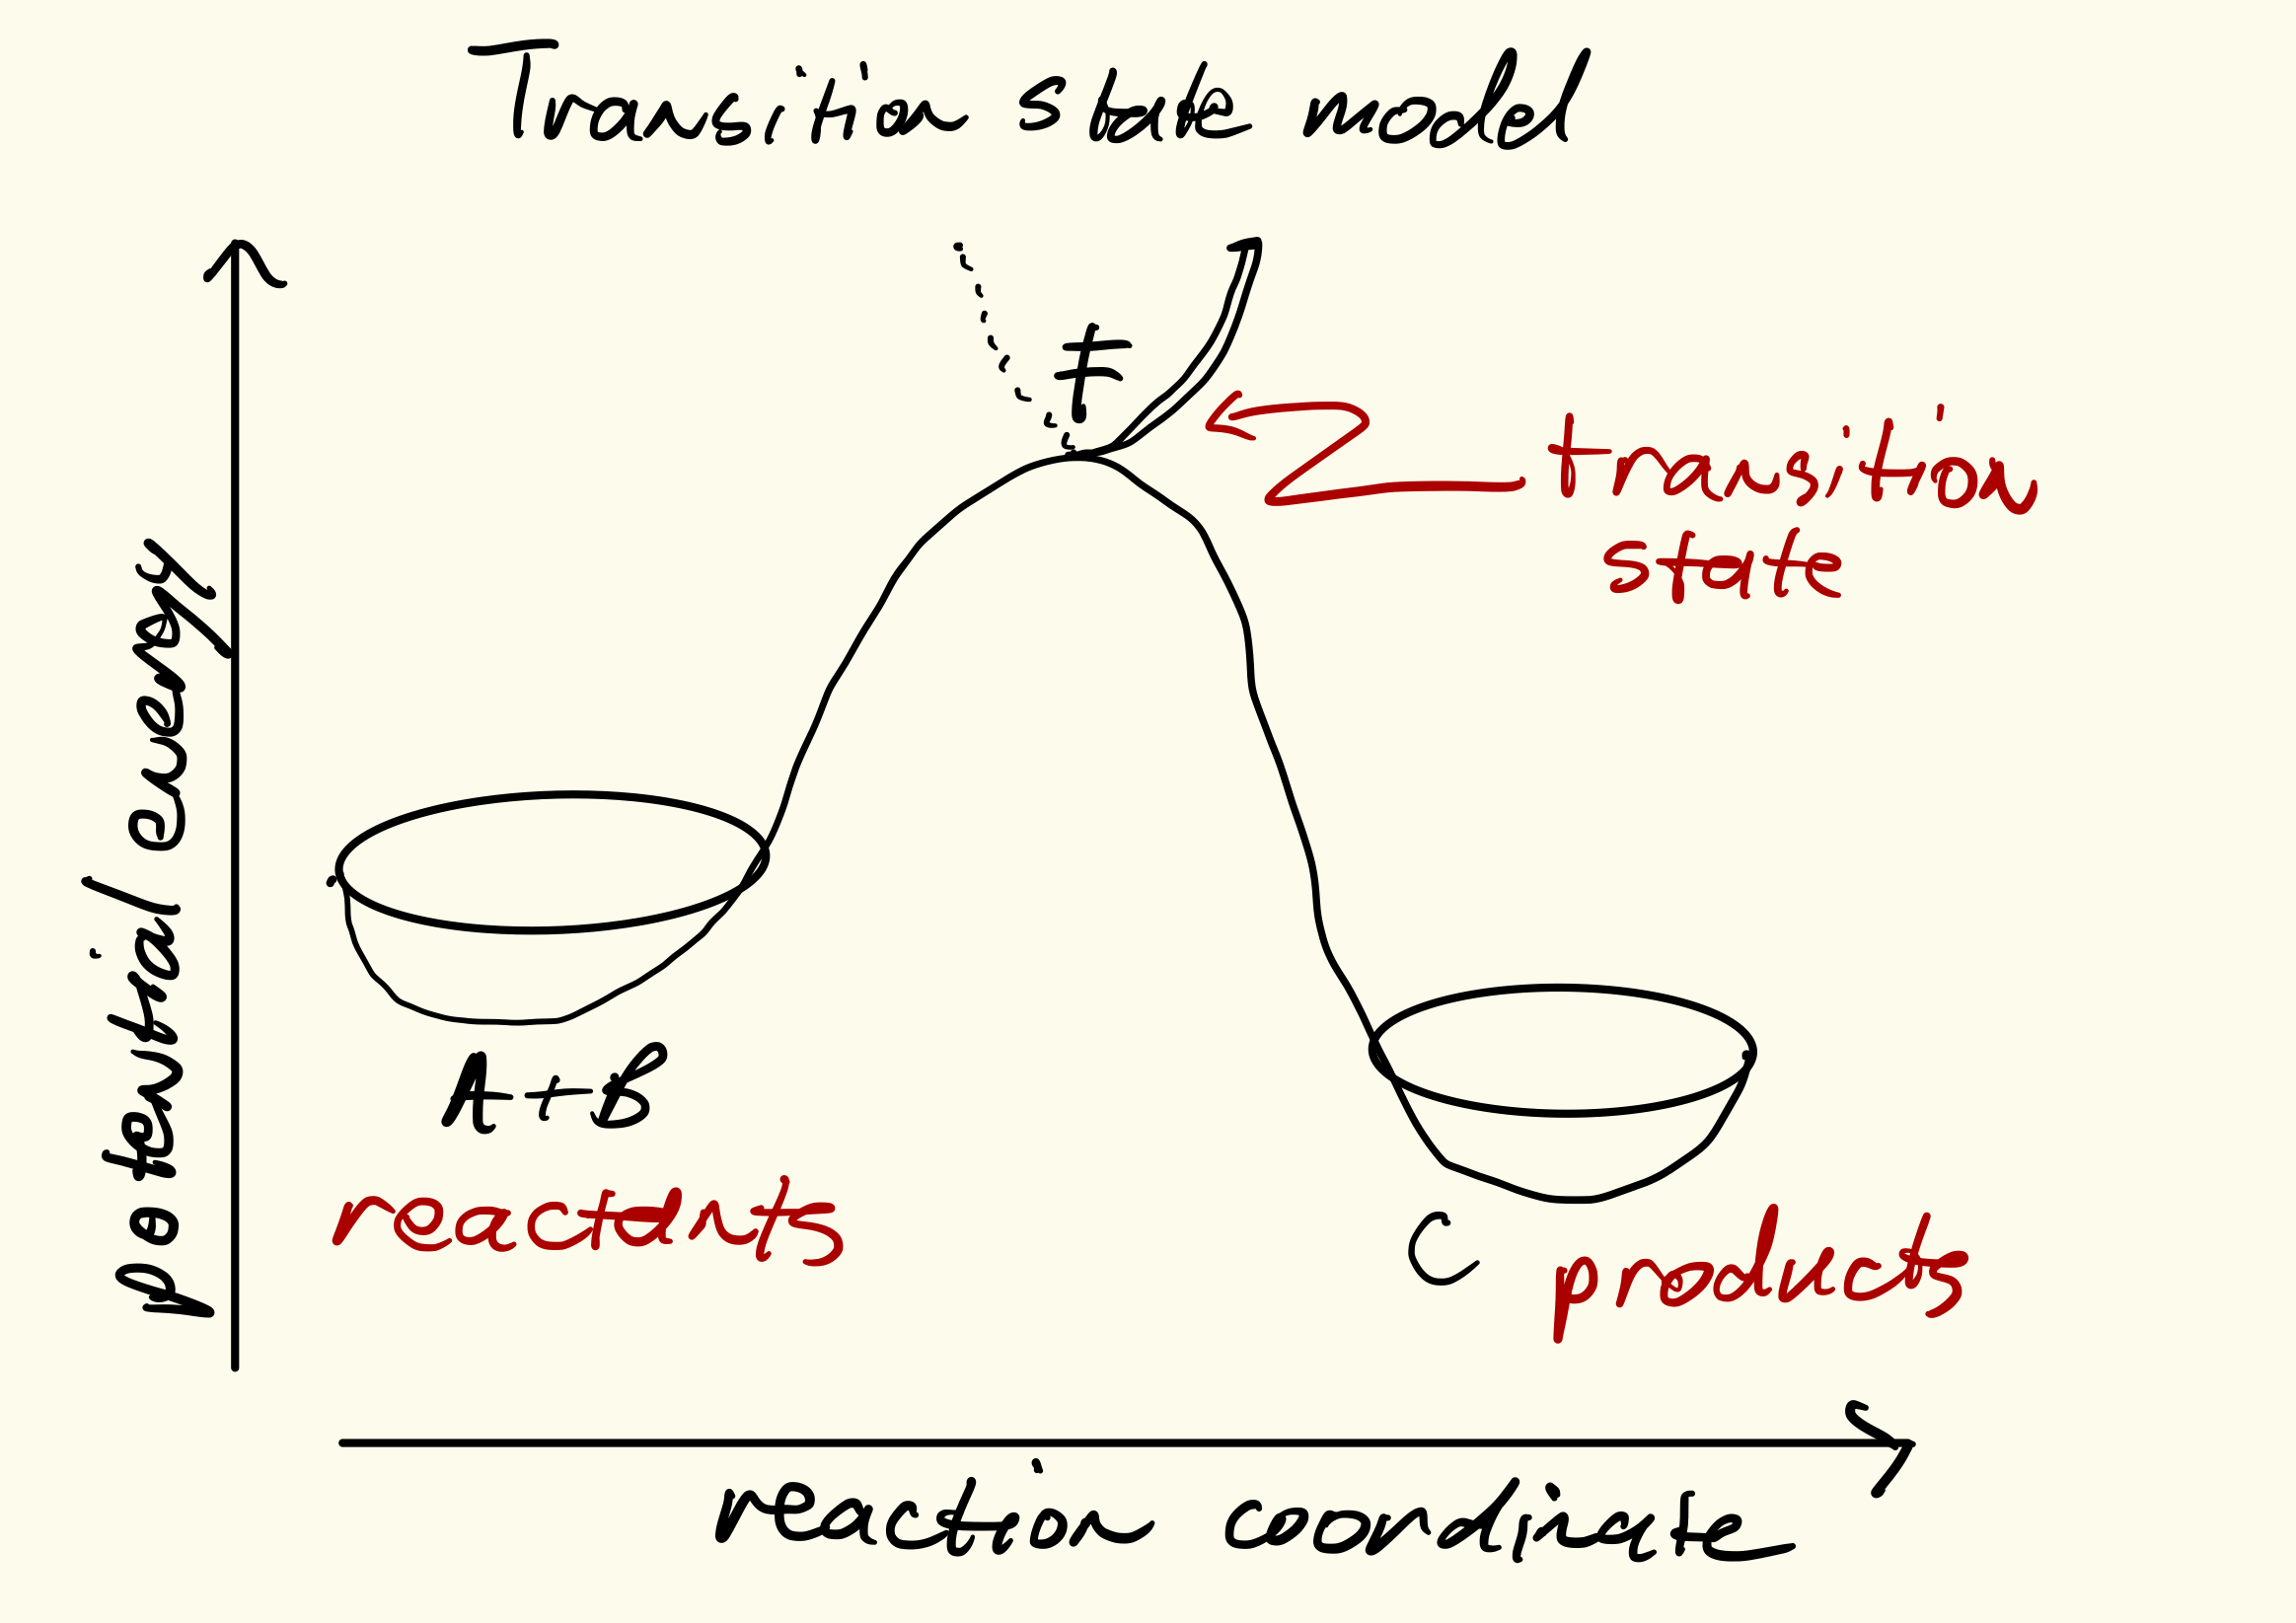
\includegraphics[width=0.6\textwidth]{./Images/PES.png}
\end{center}

\subsubsection{Locating transition states computationally}
\label{sec:org5171f58}
\subsubsection{Thermodynamic connection}
\label{sec:org6a84fd7}
\subsubsection{Diffusion-controlled reactions}
\label{sec:orgd1b849e}
\begin{enumerate}
\item Intermediate complex
\item Steady-state approximation
\item Diffusion-controlled limit (\(k_D = 4\pi (r_A + r_B) D_{AB}\))
\item Reaction-controlled limit (\(k_{app}=(k_D/k_{-D})k_r\))
\end{enumerate}

\begin{table}
\begin{center}
    \caption{\large{Equilibrium and Rate Constants}}
   \begin{description}
   \item[Equilibrium Constants] $a~\text{A} + b~\text{B} \rightleftharpoons c~\text{C} + d~\text{D} $
     \begin{eqnarray*}
       K_{eq}(T) &=& e^{\Delta S^\circ(T,V)/k_B}e^{-\Delta H^\circ(T,V)/k_BT}
       \\ \\
            K_c(T) &=&
          \left(\frac{1}{c^\circ}\right)^{\nu_c+\nu_d-\nu_a-\nu_b}\frac{(q_c/V)^{\nu_c}(q_d/V)^{\nu_d}}{(q_a/V)^{\nu_a}(q_b/V)^{\nu_b}}e^{-\Delta
            E(0)\beta}\\ \\
            K_p(T) &=&
          \left(\frac{k_BT}{P^\circ}\right)^{\nu_c+\nu_d-\nu_a-\nu_b}\frac{(q_c/V)^{\nu_c}(q_d/V)^{\nu_d}}{(q_a/V)^{\nu_a}(q_b/V)^{\nu_b}}e^{-\Delta
            E(0)\beta}
\end{eqnarray*}
\item[Unimolecular Reaction] $\text[A] \rightleftharpoons [\text{A} ]^\ddagger
  \rightarrow C$
      \begin{displaymath}
        k(T)=\nu^\ddagger \bar K^\ddagger=\frac{k_B T}{h} \frac{\bar{q}_\ddagger(T)/V}{q_A(T)/V}
          e^{-\Delta E^\ddagger(0)\beta}
      \end{displaymath}
\begin{center}
      \begin{tabular}{cc}
      $ \displaystyle E_a =\Delta H^{\circ\ddagger}+k_B T $
      & $ \displaystyle A = e^1\frac{k_B T}{h} e^{\Delta S^{\circ\ddagger}} $
      \end{tabular}
\end{center}
\item[Bimolecular Reaction] $
        \mathrm{A} + \mathrm{B} \rightleftharpoons [ \mathrm{AB}]^\ddagger
        \rightarrow \text{C}$
      \begin{displaymath}
        k(T)=\nu^\ddagger \bar K^\ddagger=\frac{k_B T}{h} \frac{q_\ddagger(T)/V}{(q_A(T)/V)(q_B(T)/V)}\left
          (\frac{1}{c^\circ}\right )^{-1}
        e^{-\Delta E^\ddagger(0)\beta}
      \end{displaymath}
      \begin{center}
        \begin{tabular}{cc}
        $ \displaystyle E_a  =\Delta H^{\circ\ddagger}+2 k_B T $ & $ \displaystyle
        A  = e^2\frac{k_B T}{h} e^{\Delta S^{\circ\ddagger}} $
      \end{tabular}
      \end{center}
   \end{description}
 \end{center}
 \end{table}

\subsection{Lecture 22: Conclusion}
\label{sec:orgce78c29}
\begin{enumerate}
\item Do you think about the burning lighter any differently now?
\end{enumerate}
\end{document}